\documentclass[a4paper,12pt]{book}
%\documentclass[a5paper,12pt,landscape]{book}
%\documentclass[a5paper,12pt,landscape]{report}

\usepackage[margin=3cm]{geometry}

\usepackage[T1]{fontenc}
\usepackage[english]{babel}
%\usepackage[utf8]{inputenc}

\usepackage{tikz}
\usetikzlibrary{calc}
\usetikzlibrary{arrows, backgrounds}
\usetikzlibrary{matrix, arrows.meta}
\usetikzlibrary{decorations.pathreplacing}

%\usepackage{amsfonts}
%\usepackage{amsmath}
%\usepackage{amsthm}
\usepackage{bm}

\usepackage{pgfplots}
\pgfplotsset{compat=1.3}
\usepgfplotslibrary{groupplots}

% Used for split environment
\usepackage{amsmath}
% Separate rows in align environment by this amount
\addtolength{\jot}{1em}

\usepackage{graphicx}
\graphicspath{{../fig/} {fig/}}
\usepackage{subfig}
\usepackage{wrapfig}

% Clickable links
\usepackage{hyperref}
\hypersetup{
	colorlinks,
	citecolor=black,
	filecolor=black,
	linkcolor=black,
	urlcolor=black
}

\usepackage[pdf]{graphviz}

%\usepackage[dvipsnames]{xcolor}
\usepackage{listings}

\lstset{
	language=c,
  basicstyle=\small\ttfamily,  % the size of the fonts that are used for the code
	numbers=none,                   % where to put the line-numbers
  inputencoding=latin1,
  numberstyle=\tiny,  % the style that is used for the line-numbers
  stepnumber=1,                   % the step between two line-numbers. If it's
				    %1, each line 
                                  % will be numbered
  %numbersep=5pt,                  % how far the line-numbers are from the code
  backgroundcolor=\color{white},      % choose the background color.
  showspaces=false,               % show spaces adding particular underscores
  showstringspaces=false,         % underline spaces within strings
  showtabs=false,      % show tabs within strings adding particular underscores
	frame=none,                   % adds a frame around the code
  rulecolor=\color{black},        % if not set, the frame-color may be changed
				   % on line-breaks within not-black text (e.g.
				   % comments (green here))
	tabsize=6,                      % sets default tabsize to 2 spaces
  columns=fullflexible,
  extendedchars=true,
  captionpos=b,                   % sets the caption-position to bottom
  breaklines=true,                % sets automatic line breaking
  breakatwhitespace=false,        % sets if automatic breaks should only happen
				    %at whitespace
  title=\lstname,                   % show the filename of files included with
				    %\lstinputlisting;
                                  % also try caption instead of title
  keywordstyle=\color{blue},          % keyword style
	commentstyle=\color{gray},       % comment style
	stringstyle=\color{brown},         % string literal style
  escapeinside={\%*}{*)},            % if you want to add LaTeX within your code
	morecomment=[l][\color{purple}]{\#},
	moredelim=[il][\color{purple}]{@},
%	abovecaptionskip=-15pt
%	belowcaptionskip=-15pt
}


\usepackage{csquotes}

\usepackage{siunitx}
\usepackage{todonotes}

\usepackage{multicol}

\usepackage{epigraph}
\setlength{\epigraphwidth}{0.7\textwidth}

\usepackage{caption}
\captionsetup{font=footnotesize}

% Macros para ayudar a la redacción
% Vector
\newcommand*\mat[1]{ \begin{pmatrix} #1 \end{pmatrix}}
\newcommand*\arr[1]{ \begin{bmatrix} #1 \end{bmatrix}}
\newcommand*\V[1]{\bm{#1}}
\newcommand{\E}{\V{E}}
\newcommand{\rhog}{\rho_\text{ghost}}
\newcommand{\F}{\V{F}}
\newcommand{\B}{\V{B}}
\renewcommand*{\v}{\V{v}}
\newcommand{\x}{\V{x}}
\newcommand{\dt}{\Delta t}
\newcommand{\dx}{\Delta x}
\newcommand*\neigh[1]{\mathcal{N}(#1)}

% Norm
\newcommand\norm[1]{\left\lVert#1\right\rVert}

\title{Particle-in-cell plasma simulation with OmpSs-2
\todo[inline]{Place proper cover page}}
\author{Rodrigo Arias Mallo}
\date{\today}

\begin{document}

\frontmatter

%\pagenumbering{roman}

% do not use titlepage environment, because it does not increase page counter.

%%%%%%%%%%%%%%%%%%%%%%%%%%%%%%%%%%%%%%%%%%%%%%%%%%%%%%%%%%
\thispagestyle{empty}
\newgeometry{left=5mm, right=5mm, bottom=5mm, top=9mm}

\begin{center}

\includegraphics[scale=0.65]{UPC.pdf}
\hspace{70mm}
\includegraphics[scale=0.65]{logofib.pdf}

\vspace{25mm}

{\bf\large Universitat Polit\`ecnica de Catalunya (UPC) - BarcelonaTech}
\par\vspace{1mm}
{\bf\large Facultat d'Inform\`atica de Barcelona (FIB)}
\par\vspace{1mm}
{\bf\large Final Master Thesis (FMT)}

\par\vspace{2mm}
{\large Master in Innovation and Research in Informatics (MIRI)}
\par\vspace{0.8mm}
{\large Advanced Computing (AC)}
\par\vspace{15mm}

%{\bf\LARGE Enhancing the Interoperability between Distributed-Memory and Task-based Programming Models}
{\bf\LARGE Particle-in-cell plasma simulation}\\
\par\vspace{0.8mm}
{\bf\LARGE with OmpSs-2}

\par\vspace{10mm}
{\bf\large Rodrigo Arias Mallo}\\
(\texttt{rodrigo.arias@bsc.es})

\vspace{10mm}

{\large Advisor:}\\
\par\vspace{1mm}
{\bf\large Vicen\c{c} Beltran Querol} (\texttt{vbeltran@bsc.es})\\
\par\vspace{3mm}
{\large Tutor:}\\
\par\vspace{1mm}
{\bf\large Jordi Torres Viñals} (\texttt{torres@ac.upc.edu}) \\
\par\vspace{4mm}

\vspace{10mm}

{\large Barcelona, 27 June 2019}

\vspace{10mm}

\begin{center}
 \includegraphics[scale=0.40]{BSCLogo.pdf}
\end{center}


\end{center}
\restoregeometry
%%%%%%%%%%%%%%%%%%%%%%%%%%%%%%%%%%%%%%%%%%%%%%%%%%%%%%%%%%%%%%%%%%%%%%%%%%%%%%%


%\newpage
\cleardoublepage

\chapter*{Abstract}
%\vspace*{\fill}
%Context
% HPC is key for scientific research
With the increasing numerical power of supercomputing facilities, High 
Performance Computing (HPC) has become key for scientific research.
% The increasing complexity makes writing programs hard
Consequently, the heterogeneous computer architectures are more complex and 
present a challenge in order to write efficient and scalable programs.
% OmpSs-2 tries to handle the complexity by offering a simple mechanism of tasks 
% annotation
The programming model provided by OmpSs-2 based in annotations in the code to 
define tasks and dependencies, unleash a new way to develop complex applications 
hiding the complications away from the programmer.
%Problem
However, it is not until a specific problem is addressed when the limitations 
and unforeseen difficulties are observed and only then new solutions can be 
proposed.

In this project, a plasma simulator is designed and parallelized using the 
task-flow model, while the different challenges found are used to propose 
improvements in the programming model.
%
As a result, a fully functional 2D electrostatic with background magnetic field 
plasma simulator is designed, based on the particle-in-cell method. A fast 
spectral and parallelized solver is included with a real-time visualization 
software.
%
The scalability is evaluated with various benchmarks and our results suggest 
that the FFT leads to a bottleneck in the simulation, from which a new proposed 
method is left to future work.



% In order to improve the methodology, a close relation with real case scenario 
% is needed

%Solution

% A plasma simulator offers the complexity needed to stress all areas of the
% computation in a scientific program.

%\vfill\cleardoublepage





\tableofcontents

%\pagenumbering{arabic}

\mainmatter

\chapter{Introduction}
\label{ch:intro}

It may be surprising to find out that the most common state of matter is plasma, 
when we look at the universe. The simulation of plasma has been increasingly 
researched since the computers began gaining computation speed, as it is quite 
complex and expensive to study in a physics laboratory. The particle-in-cell 
methods are now widely used for the simulation of different plasma phenomena, as 
they provide a good parallelization that can be exploited with today 
supercomputers.

\section{Motivation}

The design and implementation of a plasma simulator is a useful way to find out 
the patterns and complexities of a parallel application used in the real world.  
Most of the existing PIC codes are highly tied to solve a specific set of 
simulations to work on some experiments and the documentation is usually poor or 
inexistent, and the designs are the result of years added features without a 
clear design.

Using OmpSs-2 from the beginning can lead to a higher performance execution, and 
at the same time keep a clean and documented design.

\section{Objectives}

One of the main objectives of the simulation is the use of the data-flow 
execution model provided by OmpSs-2 to find the challenging computational 
patterns that occur in a complete and real application.

Furthermore the Task Aware MPI library (TAMPI), will be compared against MPI to 
measure the performance in communications on a complex simulation scenario.

The challenges found during the design of the simulator will be used to improve 
the current solutions provided by the programming model and propose new 
alternatives.

\section{Structure}
%
\begin{figure}[h]%{{{
\centering
\scalebox{0.7} {
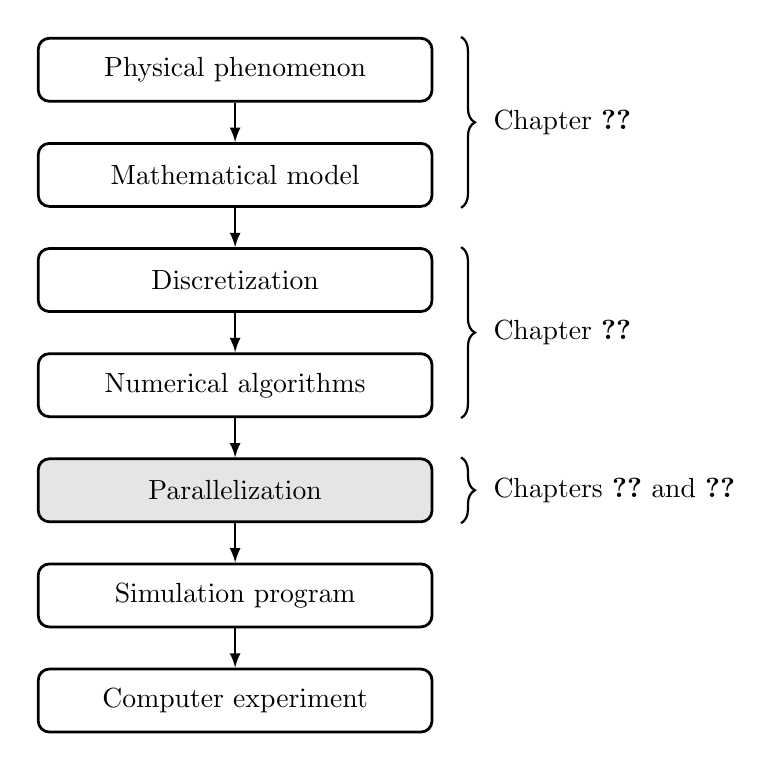
\begin{tikzpicture}[>=latex,thick]
	\matrix (m) [
		matrix of nodes,
		column sep=5mm,
		row sep=5mm,
		nodes={
			draw, % General options for all nodes
			line width=1pt,
			anchor=center,
			text centered,
			rounded corners,
			minimum width=5cm,
			minimum height=8mm,
		},
		txt/.style={text width=1.5cm,anchor=center},
	]
	{
		Physical phenomenon \\
		Mathematical model \\
		Discretization \\
		Numerical algorithms \\
		|[fill=black!10]| Parallelization \\
		Simulation program \\
		Computer experiment \\
	};
	\foreach \i [evaluate={\j=int(\i+1)}] in {1,...,6}{
		\draw[->] (m-\i-1) -- (m-\j-1);
	}
	\draw [
		decorate,decoration={brace,amplitude=5pt,raise=10pt},
	] (m-1-1.north east) -- (m-2-1.south east) node 
	[black,midway,right,xshift=18pt] {Chapter~\ref{ch:plasma-sim}};
	\draw [
		decorate,decoration={brace,amplitude=5pt,raise=10pt},
	] (m-3-1.north east) -- (m-4-1.south east) node 
	[black,midway,right,xshift=18pt] {Chapter~\ref{ch:discrete-model}};
	\draw [
		decorate,decoration={brace,amplitude=5pt,raise=10pt},
	] (m-5-1.north east) -- (m-5-1.south east) node 
	[black,midway,right,xshift=18pt]
		{Chapters~\ref{ch:parallel-simulator} and~\ref{ch:comm}};

\end{tikzpicture}
}
\caption{Principal steps in a computer simulation experiment}
\label{fig:structure}
\end{figure}%}}}
%
The structure of the document follows the diagram shown in the 
figure~\ref{fig:structure}. In the chapter~\ref{ch:plasma-sim}, plasma is 
described as a physical phenomenon and we focus on the relevant properties that 
we want to study, from which we derive a mathematical model.  The discretization 
of the model allows the computer simulation by using numerical algorithms, and 
is discussed in the chapter~\ref{ch:discrete-model}. A sequential prototype is 
designed to test the proposed model in chapter~\ref{ch:sequential}.  Then, 
following the techniques described in the chapter~\ref{ch:techniques} a parallel 
simulator is build in chapters~\ref{ch:parallel-simulator} and~\ref{ch:comm}.

Finally, the performance of the simulator is addressed in the 
chapter~\ref{ch:analysis}, leading to the conclusions and future work in the 
chapter~\ref{ch:discussion}.

%\chapter{Related work}

The simulation of plasma began with the first simulations in the 1950s with the
John Dawson codes for 1D simulation. In 1965 Hockney and Buneman introduced the
direct Poisson solver, which allowed the first useful electrostatic simulations.
In the 1970s, the theory of electrostatic PIC was developed by Langdon, leading
to the first electromagnetic codes.

Finally, from 1980 to the 90s the two main bibles of particle-in-cell codes were
produced  by B. Langdon and C. Birdsall in 1975 \cite{birdsall} and by Hockney
and Eastwood in 1988 \cite{hockney}.

At the Plasma Theory and Simulation Group of the University of California,
Berkeley the XOOPIC \cite{xoopic} family of well known codes were released in
the 1990s.

The are a lot of specific PIC codes which are currently used for the simulation
of various phenomena, mostly centered in fusion reactors: ELMFIRE, GENE, GTC,
ORB5, PAR-T and EUTERPE \cite{euterpe}.



%\part{Theory}%\\ \small \textit{No C code here}}

% What is a plasma: write about the physical phenomenon
%\chapter{Plasma introduction}
\label{ch:plasma-intro}

% Write about how plasma can be simulated with a computer. The methods regarding 
% *only* on numerical methods to simulate plasma, not the specific to HPC ones.

\section{Everyday plasmas}

It may be surprising to find out that when we look at the universe, the most
common state of matter is plasma, which is a ionized gas formed by free
electrons and ions at a region in space--often known as the fourth state of
matter. The sun, our closest star, is a giant
ball of plasma 


Most common forms of plasma only occur in vaccum, as otherwise the air cools the
plasma and returns to a gas.

In our planet, we can see forms of plasma almost every day. A storm day the
lightnings. The spark on some piezoelectric lighters, which is the very same
principle that occurs in gasoline engines.

The Aurora Borealis, of the lightning of a fluorescent tube or the pixels of a
plasma TV.

A precise definition of a plasma is given by Chen~\cite{chen} as \textit{``a
quasineutral gas of charged and neutral particles which exhibits collective
behavior''}. The 


% Begin the simulation of plasma part
\chapter{Plasma simulation}
\label{ch:plasma-sim}

% Write about how plasma can be simulated with a computer. The methods regarding 
% *only* on numerical methods to simulate plasma, not the specific to HPC ones.

\section{The particle-in-cell method}

%TODO: Show the main equation
Solving the Vaslov equation requires a large amount of numerical resources. The 
particle in cell method, approximates the solution by discretization of the 
fields.

The method is divided in four main phases: 

\begin{itemize}
\item Particle motion.
\item Charge accumulation.
\item Solve field equation.
\item Interpolation of fields in particle position.
\end{itemize}


%\section{1D electrostatic simulation}
%The magnetic field is ignored.
%
%\section{2D simulation}
%The magnetic field is not ignored.
%
%\section{Electromagnetism}
%
%\subsection{Background magnetic field}
%
%To introduce the magnetic field, the equations are:
%
%$$ $$

\section{Particle mover}

In order to move the particles, the equations of motion need to be solved:
%
\begin{equation}
m \frac{d\v}{dt} = q (\E + \v \times \B)
\end{equation}
\begin{equation}
\frac{d\v}{dt}=\v
\end{equation}
%
Several methods are available, but we will focus on the Boris integrator.

\subsection{Boris integrator}

Consists of three steps:
%
\begin{enumerate}
\item Add half of the electric impulse
\item Rotate
\item Add the remaining half electric impulse
\end{enumerate}
%
The Boris integrator computes the velocity of a particle in a constant electric 
field $\E$ and a constant magnetic field $\B$. We have the velocity 
$\v_{t-\Delta t/2}$ of the particle at $t-\Delta t/2$ as we use the leapfrog 
integrator.
%
\begin{figure}[h]
\centering
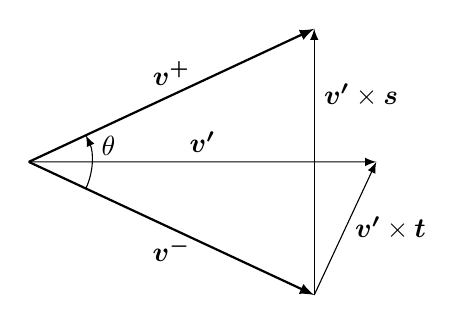
\begin{tikzpicture}[
	scale=2,
	>=latex]

	\def\centerarc[#1](#2)(#3:#4:#5)% Syntax: [draw options] (center) (initial angle:final angle:radius)
		{\draw[#1] ($(#2)+({#5*cos(#3)},{#5*sin(#3)})$) arc (#3:#4:#5); }

	\def\startangle{-25}
	\def\midangle{0}
	\def\endangle{25}
	\def\radius{2.0}
	\pgfmathsetmacro{\vlen}{\radius*tan(\startangle)}%

	\coordinate (O) at (0,0);
	\coordinate (S) at (\startangle:\radius);
	\coordinate (E) at (\endangle:\radius);

%	\centerarc[dashed](O)(\startangle:\endangle:\radius);
	\centerarc[->](O)(\startangle:\endangle:0.2*\radius);

	\draw (O)+(0.4,0.1) node [right] {$\theta$};

	\draw [thick,->] (O) -- (E) node [midway, above] {$\V{v^+}$};
	\draw [thick,->] (O) -- (S) node [midway, below] {$\V{v^-}$};

	\path (S) +(\startangle-90:\vlen) coordinate (V1E);
%	\path (E) +(\endangle-90:\vlen) coordinate (V3E);

%	%\draw [->] (E) -- (V3E);
	\draw [->] (S) -- (V1E) node [midway, right] {$\V{v'} \times \V t$};
%
	\draw [->] (O) -- (V1E) node [midway, above] {$\V{v'}$};
	\draw [->] (S) -- (E) node [near end, right] {$\V{v'} \times \V s$};

%	\draw [fill=white] (O) circle (0.02);

\end{tikzpicture}
\caption{Velocity space rotation from $\v-$ to $\v+$}
\end{figure}
%
\paragraph{Add half electric impulse} We define $\V{v^-}$ as the velocity after 
half a electric impulse:
$$\v^- = \v_{t-\dt/2} + \frac{q \E}{m} \frac{\dt}{2}$$

\paragraph{Rotate for the magnetic field} The rotation is done in two steps, 
first the half rotation is computed, with an angle of $\theta/2$:
$$\v' = \v^- + \v^- \times \V t $$

Then the rotation is completed by symmetry, using the $\V s$ vector
$$ \V s = \frac{2 \V t}{1 + \V t^2} $$
as
$$ \V{v^+} = \V{v^-} + \V{v}' \times \V{s} $$

\section{Charge accumulation}

The charge density $\rho$ is a scalar field

\section{Field equations}

Once we have the charge density $\rho$ we can compute the electric field $\E$ by 
the integration of the field equations
%
\begin{equation}
\E = -\nabla \phi
\end{equation}
\begin{equation}
\nabla \cdot \E = \frac{\rho}{\epsilon_0}
\end{equation}
%
Which can be combined into the Poisson equation
%
\begin{equation}
\label{eq:poisson}
\nabla^2\phi = - \frac{\rho}{\epsilon_0}
\end{equation}
%
Different methods can be used to obtain the electric field, but we will focus on 
matrix and spectral methods.


\chapter{Discrete model}
\label{ch:discrete-model}

\epigraph{... all models are approximations. Essentially, all models are wrong, but some
are useful. However, the approximate nature of the model must always be borne in
mind....}{Empirical Model-Building and Response Surfaces, 1987---George E. P.  
Box}

The mathematical model is discretized in algebraic operations, in order to be 
computable.

\section{Charge assignment}
At each grid point $g$ at $\x$ we accumulate the charge of each particle $p$ in 
$\x_p$ as
%
\begin{equation}%{{{
\rho(\x) = \sum_p q\,W(\x - \x_p) + \rho_0
\end{equation}%}}}
%
The background charge density $\rho_0$ is used to neutralize the total charge 
when is non-zero. The weighting function $W$ determines the shape of the 
particle charge. Different schemes can be used to approximate the charge density 
from the particles. We will focus on bilinear interpolation for it's simplicity 
and low computation requirements. The corresponding weighting function can be 
written as
%
\begin{equation}%{{{
W(\x) =
\begin{cases}
			\displaystyle\left(1 - \frac{|x|}{\Delta x}\right)
				\left(1 - \frac{|y|}{\Delta y}\right) & \text{if}\ -\Delta\x < \x < 
				\Delta \x\\
			0 & \text{otherwise}
\end{cases}
\end{equation}%}}}
%
Notice that a particle $p$ always affects the four enclosing grid points in the 
neighbourhood $\neigh{p}$, but more complex interpolation methods may extend the 
update region even further. It may be noted that the increase in smoothing, at 
computation expense, can gain from the reduced number of particles needed to 
obtain a similar result, avoiding nonphysical effects.
%
\begin{figure}[]%{{{
\centering
\begin{tikzpicture}[
		>=latex,
		effect/.style={dashed,-{Latex[length=3mm, width=1mm]}},
		particle/.style={fill=black,radius=3pt},
	]
	\draw [step=2cm,dotted] (1,1) grid (5,5);
	\coordinate (p) at (2.5,3.2);
	\coordinate (center) at (3,3);
	\coordinate (A) at ($(center)+(-1,1)$);
	\coordinate (B) at ($(center)+(1,1)$);
	\coordinate (C) at ($(center)+(1,-1)$);
	\coordinate (D) at ($(center)+(-1,-1)$);
	\draw[effect] (p) -- (A);
	\draw[effect] (p) -- (B);
	\draw[effect] (p) -- (C);
	\draw[effect] (p) -- (D);
	\node[above left]  at (A) {$A$};
	\node[above right] at (B) {$B$};
	\node[below right] at (C) {$C$};
	\node[below left]  at (D) {$D$};
	\draw[particle] (p) circle;
	\node[left] at (p) {$p$};
\end{tikzpicture}
\hspace{0.5cm}
\begin{tikzpicture}[
		>=latex,
		box/.style={black},
		particle/.style={fill=black,radius=3pt},
		div/.style={dashed},
	]
	\draw [step=2cm,dotted] (1,1) grid (5,5);
	\coordinate (p) at (2.5,3.2);
	\coordinate (center) at (3,3);
	\coordinate (A) at ($(p)+(-1,1)$);
	\coordinate (B) at ($(p)+(1,1)$);
	\coordinate (C) at ($(p)+(1,-1)$);
	\coordinate (D) at ($(p)+(-1,-1)$);
	\draw[box] (A) -- (B) -- (C) -- (D) -- (A);
	\draw[div] ($(A)!(center)!(B)$) -- (center);
	\draw[div] ($(B)!(center)!(C)$) -- (center);
	\draw[div] ($(C)!(center)!(D)$) -- (center);
	\draw[div] ($(D)!(center)!(A)$) -- (center);
	\node at ($(center)!0.5!(A)$) {$a$};
	\node at ($(center)!0.5!(B)$) {$b$};
	\node at ($(center)!0.5!(C)$) {$c$};
	\node at ($(center)!0.5!(D)$) {$d$};
	\draw[particle] (p) circle;
\end{tikzpicture}
\hspace{0.5cm}
\begin{tikzpicture}[
		>=latex,
		box/.style={black},
		particle/.style={fill=black,radius=3pt},
		div/.style={dashed},
	]
	\draw [step=2cm,dotted] (1,1) grid (5,5);
	\coordinate (p) at (2.5,3.2);
	\coordinate (center) at (3,3);
	\coordinate (A) at ($(center)+(-1,1)$);
	\coordinate (B) at ($(center)+(1,1)$);
	\coordinate (C) at ($(center)+(1,-1)$);
	\coordinate (D) at ($(center)+(-1,-1)$);
	\draw[box] (A) -- (B) -- (C) -- (D) -- (A);
	\draw[div] ($(A)!(p)!(B)$) -- (p);
	\draw[div] ($(B)!(p)!(C)$) -- (p);
	\draw[div] ($(C)!(p)!(D)$) -- (p);
	\draw[div] ($(D)!(p)!(A)$) -- (p);
	\node at ($(p)!0.5!(A)$) {$c$};
	\node at ($(p)!0.5!(B)$) {$d$};
	\node at ($(p)!0.5!(C)$) {$a$};
	\node at ($(p)!0.5!(D)$) {$b$};
	\draw[particle] (p) circle;
\end{tikzpicture}
\caption{Interpolation of particle $p$ charge into the four grid points A to D.}
\label{fig:interpolation}
\end{figure}%}}}
%
The particle $p$ has a uniform charge area, centered at the particle position 
$\x_p$, with size $\Delta \x$, as shown in the figure~\ref{fig:interpolation}.  
Each grid point $A,B,C$ and $D$ receives the amount of charge weighed by the 
area $a,b,c$ and $d$. It can be observed that the area is equal to the opposite 
region, when the particle $p$ is used to divide the grid cell.
%
The particle shape can be altered later in the Fourier space, without large 
computation effort, in case the solver already computes the FFT.
%
\section{Field equations}

In order to compute the electric field $\E$, the electric potential $\phi$ is 
generally needed, which can be obtained from the charge density $\rho$.

\subsection{Electric potential}
Several methods are available to solve the Poisson equation 
(Eq.~\ref{eq:poisson}).

\paragraph{Iterative  methods} such as Jacobi, Gauss-Seidel, Successive Over 
Relaxation (SOR), Chebyshev acceleration are some of the most familiar methods 
to solve the Poisson equation.

\paragraph{Matrix methods} The equations from finite differencing the mesh are 
considered a large system of equations. We can find in this methods the Thomas 
Tridiagonal algorithm, Conjugate-Gradient, LU or Incomplete Decomposition.

\paragraph{Spectral methods} Also known as Rapid Elliptic Solvers (RES) are a 
family of methods that use the fast Fourier transform (FFT). Are know for being 
usually faster than the previous ones, with a complexity in $O(N_g \log_2 N_g)$

\vspace{1em}
\noindent
%
We will only focus on the LU for small problems and for testing, and spectral 
methods, more specific on the Multiple Fourier Transform (MTF) method, as it is 
the main method implemented in the simulator, due to its relative simplicity and 
low computational complexity.

\subsection{LU decomposition}
%
% TODO: Check the error bound
For two dimensions, we can approximate the solution using the second order 
centered finite differences (with an error proportional to $\Delta x ^2 \Delta 
y^2$), as
%
\begin{equation}%{{{
\label{eq:discrete-poisson}
\frac{\phi(x-1, y) + \phi(x, y-1) - 4\phi(x,y) + \phi(x+1,y)+\phi(x,y+1)}{\Delta 
x ^2 \Delta y^2} = - \frac{\rho(x,y)}{\epsilon_0}
\end{equation}%}}}
%
which leads to a system of $N_g$ linear equations and can be also written in 
matrix form
%
\begin{equation}
\label{eq:eq-system}
A\phi = -\frac{\Delta x ^2 \Delta y^2\,\rho}{\epsilon_0}
\end{equation}
%
The $N_g \times N_g$ coefficient matrix $A$ has non-zero coefficients only at 
$a_{ii} = 4$ and $a_{ij} = -1$ with $j \in \{i+1, i-1, i+N_x, i-N_x\} \mod N_x$, 
for all $0 \le i \le Ng$.
%
However, the matrix $A$ is singular, so the system of equations has infinite 
solutions. Boundary conditions can be added to get a unique solution. The extra 
equation $\phi(0,0) = 0$ leads to a system with only one solution, but with one 
extra equation. In order to keep the matrix $A$ square, the following steps may 
be taken:

\begin{enumerate}
\item Subtract  the extra equation $\phi(0,0) = 0$ to the first row of $A$, with 
the only change in the coefficient to $a_{11} = 3$.

\item Add all first $N_g$ equations: Each equation has one coefficient of $4$ 
and four of $-1$ except the first equation. Also we assume the total charge 
density is zero, obtaining $\phi(0,0) = 0$.

\item Subtract it from the last equation, which leads to a zero coefficient that 
can be removed.
\end{enumerate}
%
The only change that remains is at the coefficient $a_{11} = 3$. Now the matrix 
$A$ is squared and non-singular and has only one solution and can now be solved 
with the $LU$ method.

The $LU$ decomposition, with a complexity in $O(2/3N_g^3)$, can be used to form 
two systems of equations that can be solved faster. If we rewrite the system of 
equations~\ref{eq:eq-system} as the usual form $Ax=b$ with
\begin{equation}
x = \phi,\quad b = -\frac{\Delta x ^2 \Delta y^2\,\rho}{\epsilon_0}
\end{equation}
%
Then we can use the decomposition $A=LU$ to form two systems of equations
%
\begin{equation}
\label{eq:LU-systems}
Ux=y, \quad Ly=b
\end{equation}
%
which can be solved in complexity $O(2N_g^2)$.


\subsection{Multiple Fourier Transform (MFT)}

The general second-order PDE with constant coefficients and periodic boundary 
conditions
%
\begin{equation}%{{{
\label{eq:gen-fd}
a \frac{\partial^2 \phi}{\partial x^2}+b\frac{\partial \phi}{\partial x}+c\phi +
d \frac{\partial^2 \phi}{\partial y^2}+e\frac{\partial \phi}{\partial y}+f\phi = 
g(x,y)
\end{equation}%}}}
%
can be solved by using the FFT. If we expand $\phi$ and $g$ in a finite double 
Fourier series, we obtain
%
\begin{equation}%{{{
\phi(x,y) = \sum_{k,l} \hat \phi(k, l) \exp\left({\frac{2\pi i (xk + 
yl)}{n}}\right)
\end{equation}%}}}
%
and
%
\begin{equation}%{{{
g(x,y) = \sum_{k,l} \hat g(k, l) \exp\left({\frac{2\pi i (xk + yl)}{n}}\right)
\end{equation}%}}}
%
which now can be substituted in the Eq.~\ref{eq:gen-fd}, to obtain
%
\begin{equation}%{{{
\hat \phi(k,l) = \hat G(k,l) \, \hat g(k,l),\quad 0<k<N_x,\,0<l<N_y
\end{equation}%}}}
%
with for a unit mesh
%
\begin{equation}%{{{
\begin{split}
\hat G(k,l) = \Bigg[
& 2a \left( \cos \frac{2\pi k}{n} - 1 \right) +
ib \sin \frac{2\pi k}{n} + c \,+ \\
& 2d \left( \cos \frac{2\pi l}{n} - 1 \right) +
ie \sin \frac{2\pi l}{n} + f
\Bigg]^{-1}
\end{split}
\end{equation}%}}}
%
To solve the Poisson equation, discretized as Eq.~\ref{eq:discrete-poisson}, we 
have $a=d=1$ and $b=c=e=f=0$ so we can simplify $\hat G(k,l)$ as
%
\begin{equation}%{{{
\hat G(k,l) = \frac{1}{2}\left[
\cos \frac{2\pi k}{n} +
\cos \frac{2\pi l}{n} -
2 \right]^{-1}
\end{equation}%}}}
%
Let $g = -{\Delta x ^2 \Delta y^2\,\rho}/{\epsilon_0}$, then the steps to 
compute the electric potential can be summarized as follows:
%
\begin{center}%{{{
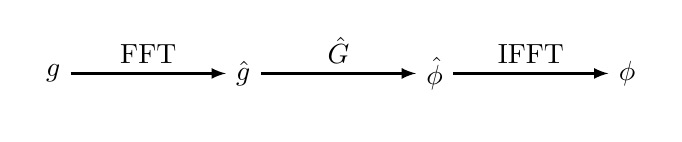
\begin{tikzpicture}[>=latex,thick]
	\matrix (m) [
		matrix of nodes,
		column sep=20mm,
		nodes={
			%line width=1pt,
			anchor=center,
			text centered,
			%minimum width=1cm,
			minimum height=8mm,
		},
%		txt/.style={text width=1.5cm,anchor=center},
	]
	{
		$g$ & $\hat g$ & $\hat \phi$ & $\phi$ \\%& $\E$\\
	};
	\foreach \i [evaluate={\j=int(\i+1)}] in {1,...,3}{
		\draw[->] (m-1-\i) -- (m-1-\j);
	}
	\draw[draw=none] (m-1-1) -- (m-1-2) node[midway,above] {FFT};
	\draw[draw=none] (m-1-2) -- (m-1-3) node[midway,above] {$\hat G$};
	\draw[draw=none] (m-1-3) -- (m-1-4) node[midway,above] {IFFT};
%	\draw[draw=none] (m-1-4) -- (m-1-5) node[midway,above]
%	{Eq.~\ref{eq:phi-to-E}};
\end{tikzpicture}
\end{center}%}}}
%
\begin{enumerate}
\item Compute the complex FFT $\hat g$ of $g$
\item Multiply each element of $\hat g$ by the corresponding complex coefficient 
$\hat G$, to obtain $\hat \phi$
\item Compute the inverse FFT of $\hat \phi$ to get $\phi$
\end{enumerate}
%
The complexity in the worst case is in $O(N_g \log_2 N_g)$ with the number of 
total points in the grid $N_g$.

\subsection{Electric field}
The electric field $\E$ can then be obtained by centered first order finite 
differences in each dimension
%
\begin{equation}%{{{
\begin{split}
\label{eq:phi-to-E}
\E_x(x,y) &= \frac{\phi(x-1,y) - \phi(x+1,y)}{2\,\Delta x} \\
\E_y(x,y) &= \frac{\phi(x,y-1) - \phi(x,y+1)}{2\,\Delta y}
\end{split}
\end{equation}%}}}
%

\section{Force interpolation}

The force acting on a particle $p$ can be decomposed in two main parts, the 
electric and magnetic force $\F=\F_E + \F_B$.

The electric force $\F_E$ is computed similarly as the charge deposition, but in 
the reverse order. The force $\F_E$ is interpolated from the electric field $\E$ 
of the neighbour grid points $\neigh{p}$, using the same interpolation function 
$W$.
\begin{equation}%{{{
\begin{split}
\F_E &= q \sum_{g \in \neigh{p}} W(\x_p - \x_g)\ \E(\x_g) \\
\end{split}
\end{equation}%}}}
Notice that a particle $p$ only needs the values of the electric field in the 
neighbourhood $\neigh{p}$.

The magnetic force $\F_B$ is constant in the simulator, as we only consider a 
fixed background magnetic field $\B_0$. For a particle $p$ with velocity $\v$  
can be written as
%
\begin{equation}%{{{
\F_B = q (\v \times \B_0)
\end{equation}%}}}


\section{Equations of motion}

In order to move the particles, the equations of motion need to be solved:
%
\begin{equation}
\frac{d\x}{dt}=\v
\end{equation}
\begin{equation}
m \frac{d\v}{dt} = \F
\end{equation}
%
The \textit{leap-frog} method is a common integration scheme with second-order 
accuracy and an error proportional to $\Delta t^2$. The name describes de 
behavior of the position and velocity, which are updated at interleaved time 
steps, similarly to the trajectory of a frog. The method is time reversible with 
an stability far superior of other higher-order integration methods, such as 
fourth order Runge-Kutta. A more in depth stability analysis can be found in 
Chapter 4 of Hockney and Eastwood book~\cite{hockney}.  The discretized 
equations can be written as
%
\begin{equation}
\frac{\x^{n+1} - \x^{n}}{\Delta \x} = \v^{n + 1/2}
\end{equation}
%
\begin{equation}
m\frac{\v^{n+1/2} - \v^{n-1/2}}{\Delta \x} = \F(x^n)
\end{equation}
%
Several methods are available, but we will focus on the Boris integrator.

\subsection{Boris integrator}

Consists of three steps:
%
\begin{enumerate}
\item Add half of the electric impulse
\item Rotate
\item Add the remaining half electric impulse
\end{enumerate}
%
The Boris integrator computes the velocity of a particle in a constant electric 
field $\E$ and a constant magnetic field $\B$. We have the velocity 
$\v_{t-\Delta t/2}$ of the particle at $t-\Delta t/2$ as we use the leapfrog 
integrator.
%
\begin{figure}[h]
\centering
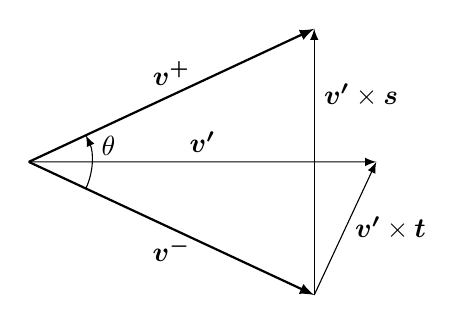
\begin{tikzpicture}[
	scale=2,
	>=latex]

	\def\centerarc[#1](#2)(#3:#4:#5)% Syntax: [draw options] (center) (initial angle:final angle:radius)
		{\draw[#1] ($(#2)+({#5*cos(#3)},{#5*sin(#3)})$) arc (#3:#4:#5); }

	\def\startangle{-25}
	\def\midangle{0}
	\def\endangle{25}
	\def\radius{2.0}
	\pgfmathsetmacro{\vlen}{\radius*tan(\startangle)}%

	\coordinate (O) at (0,0);
	\coordinate (S) at (\startangle:\radius);
	\coordinate (E) at (\endangle:\radius);

%	\centerarc[dashed](O)(\startangle:\endangle:\radius);
	\centerarc[->](O)(\startangle:\endangle:0.2*\radius);

	\draw (O)+(0.4,0.1) node [right] {$\theta$};

	\draw [thick,->] (O) -- (E) node [midway, above] {$\V{v^+}$};
	\draw [thick,->] (O) -- (S) node [midway, below] {$\V{v^-}$};

	\path (S) +(\startangle-90:\vlen) coordinate (V1E);
%	\path (E) +(\endangle-90:\vlen) coordinate (V3E);

%	%\draw [->] (E) -- (V3E);
	\draw [->] (S) -- (V1E) node [midway, right] {$\V{v'} \times \V t$};
%
	\draw [->] (O) -- (V1E) node [midway, above] {$\V{v'}$};
	\draw [->] (S) -- (E) node [near end, right] {$\V{v'} \times \V s$};

%	\draw [fill=white] (O) circle (0.02);

\end{tikzpicture}
\caption{Velocity space rotation from $\v-$ to $\v+$}
\end{figure}
%
\paragraph{Add half electric impulse} We define $\V{v^-}$ as the velocity after 
half a electric impulse:
$$\v^- = \v_{t-\dt/2} + \frac{q \E}{m} \frac{\dt}{2}$$

\paragraph{Rotate for the magnetic field} The rotation is done in two steps, 
first the half rotation is computed, with an angle of $\theta/2$:
$$\v' = \v^- + \v^- \times \V t $$

Then the rotation is completed by symmetry, using the $\V s$ vector
$$ \V s = \frac{2 \V t}{1 + \V t^2} $$
as
$$ \V{v^+} = \V{v^-} + \V{v}' \times \V{s} $$


%\part{Computation}%\\ \small \textit{No more physics now}}

\input{ch/sequential.tex}
\chapter{Parallelization techniques}
\label{ch:techniques}

\section{Message Passing Interface}

From the need of standarize communications in a distributed computing
environment, the first draft was proposed in 1992 at the Workshop on Standards
for Message Passing in a Distributed Memory Environment, and has now become one
of the most used communication protocol in HPC. The Message Passing Interface
(MPI) provides a simple to use set of routines to allow processes distributed
among different nodes to comunicate efficiently.

\subsection{Concepts}


\paragraph{Communicator} A communicator refers to a group of processes, in which
each has assigned a unique identifier called the \textit{rank}.

\paragraph{Point-to-point communication} In order for a process to exchange
information with another process, the MPI standard defines what are called
point-to-point communication routines. The most common examples are
\texttt{MPI\_Send} to send data, and \texttt{MPI\_Recv} for the reception.
Both routines need the rank of the process to stablish the connection.
Additionally a tag is used to label each message, which can be specified in the
reception to filter other messages.

\paragraph{Blocking communication} The standard defines various types of
communication methods for sending and receiving data. The so called blocking
routines are designed such that the call does not return until the communication
has been done. In the \texttt{MPI\_Send} case, the call returns when the sending
data can be safely modified, as has been sent or buffered. In the case of
\texttt{MPI\_Recv} the routine only returns when the data has been received.

\paragraph{Non-blocking communication} Similarly as with the blocking
communication, the routines \texttt{MPI\_Isend} and \texttt{MPI\_Irecv} don't
wait until the message is sent or received to return. They return inmediately,
and the communication status can be checked with \texttt{MPI\_Test} or the
process can wait until the communication request has finished with
\texttt{MPI\_Wait}.

\section{OmpSs-2}

OmpSs-2 is the next generation of the OmpSs programming model, composed of a set
of directives and library routines. It combines the OpenMP-like incremental 
parallelization approach, by means of source code annotations, with the StarSs 
execution model, based on a thread-pool design pattern.

\subsection{Concepts}

\paragraph{Task} In OmpSs-2 a task is a section of code that can be executed
independently by the runtime scheduler. Tasks may have associated dependencies
which lets the scheduler determine in which order they must be executed.  The 
notation used to describe a task is by the utilization of the
\texttt{\#pragma oss} directive, for example:
%
\begin{lstlisting}
#pragma oss task out(a[0:N-1]) label(Task 1)
for(i=0; i < N; i++)
	a[i] = 3.0 * i;

#pragma oss task inout(a[0:N-1]) in(b[0:N-1]) label(Task 2)
for(i=0; i < N; i++)
	a[i] += b[i];
\end{lstlisting}
%
The task 1 writes to the vector \texttt{a} and is stated explicitly by the 
\texttt{out} directive. Then, the task 2 will need the values of the vector 
\texttt{a}, so the execution must wait until the task 1 finishes.

\paragraph{Parallel execution} Unless there is a unmet dependency, all tasks 
ready to run are executed in parallel, up to the number of CPU cores available 
to the runtime.

\paragraph{Task syncronization} It may be possible that at some point in the
execution all pending tasks are required to finish in order to continue. The
directive \texttt{taskwait} allows the programmer to specify that the current 
task must wait for completion of all the previously created tasks.

\section{TAMPI}

The Task-Aware MPI or TAMPI library provides interoperability between OmpSs-2 
and the MPI message passing library, in order to avoid deadlocks and improve 
performance. Two modes of operations are available: blocking and non-blocking 
mode.

\subsection{Blocking mode}

When a call to a MPI function cannot be complete immediately, the task is paused 
and other task can begin the execution. As soon as the operation completes, the 
task is resumed to continue the execution. The main functions \texttt{MPI\_Recv} 
and \texttt{MPI\_Send} support this mode, from the many more available in TAMPI.  

\subsection{Non-blocking mode}

This mode is focused on the family of non-blocking MPI operations, which return 
immediately. The two functions \texttt{TAMPI\_Iwait} and 
\texttt{TAMPI\_Iwaitall} are introduced with a special behaviour: once called, 
they return immediately and the task continues the execution until the end. But 
the completion of the task is delayed until all the communications are 
completed.


%\chapter{Simulator design}

[This chapter will be merged with the next one, is only here to keep the
numbering of the chapters, while I'm working on the comments]

\chapter{The simulator}
\label{ch:parallel-simulator}

\section{Decomposition}

To parallelize the simulation, the process must be decomposed in parts that can 
be executed in parallel and several decompositions are known.
%
One of the most common technique found in particle-in-cell codes, is the 
\textit{domain decomposition}---the physical space is divided into sections of 
similar size and the fields are assigned to different computing units. The main 
drawback of this technique is the risk of unbalanced load, as some regions of 
space may contain a large amount or even all the particles.

Another approach called \textit{particle decomposition} consists in the division 
of the particles into groups, where each processor maintains a copy of the 
fields of the whole space.  The problem of this method is the limitation of 
scalability, as the number of grid points used in the fields is limited by the 
memory of one computing element.

Additionally, the Fourier transform needed by the MFT solver is implemented 
using the FFTW library and the parallelization design provided by the library 
introduces a constraint in the distribution of the fields: they need to be 
broken into slices in the Y dimension, resulting in contiguous blocks of 
elements in X. Consequently, the domain decomposition is the chosen technique 
for the simulator.

\begin{figure}[ht]%{{{
\centering
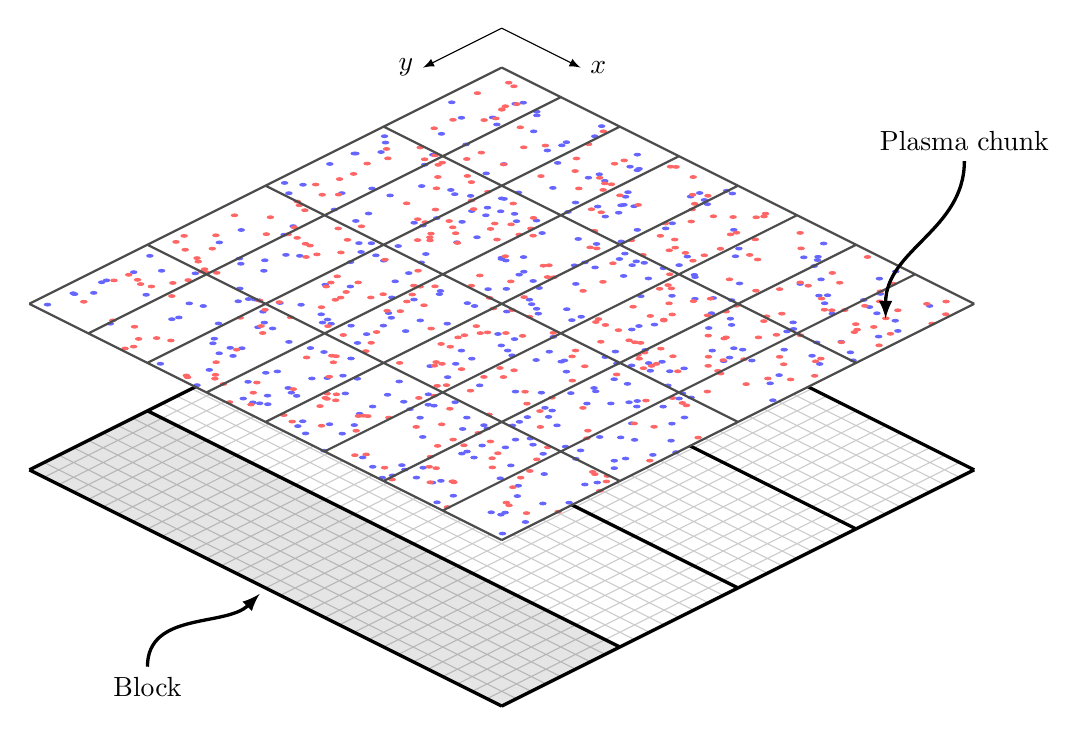
\begin{tikzpicture}
\begin{scope}[
		x=1cm,
		y=1cm,
		yshift=0,
		every node/.append style={
			yslant=0.5,xslant=-1},
		yslant=0.5,
		xslant=-1
	]
	% opacity to prevent graphical interference
	\draw[step=1.5/8, black!20!white, thin] (0,0) grid (6,6); %defining grids
	%\draw[step=1.5, black] (0,0) grid (6,6);
	\draw[xstep=1.5, ystep=6, black, very thick] (0,0) grid (6,6);
	%\draw[dashed, xstep=6, ystep=1.5, black] (0,0) grid (6,6);
	\fill[fill=black,fill opacity=0.1] (0,0) rectangle (1.5,6);
	\coordinate (a0) at (4.5, 0);
	\coordinate (a1) at (6, 0);
	\coordinate (a2) at (4.5, 1.5);
	\coordinate (a3) at (6, 1.5);

	\coordinate (b) at (0,3);

\end{scope}
\begin{scope}[
		x=1cm,
		y=1cm,
		yshift=60,
		every node/.append style={
			yslant=0.5,xslant=-1},
		yslant=0.5,
		xslant=-1
	]
	\coordinate (b0) at (4.5, 0);
	\coordinate (b1) at (6, 0);
	\coordinate (b2) at (4.5, 1.5);
	\coordinate (b3) at (6, 1.5);
	\coordinate (c) at (4.5+0.75, 0.75/2);
	%Idem as above, for the n-th grid:
%	\draw[dotted] (a0) -- (b0);
%	\draw[dotted] (a1) -- (b1);
%	\draw[dotted] (a2) -- (b2);
%	\draw[dotted] (a3) -- (b3);
%
%	\draw[dashed] (a2) -- (a3);

	\fill[fill=white,fill opacity=1.0] (0,0) rectangle (6,6);
	\begin{axis}[width=7.5cm,height=7.5cm,
						axis lines=none,
						%hide axis,
						xmin=-1, xmax=1,
						ymin=-1, ymax=1,
						inner frame sep=0,
				]
	\addplot [blue!60!white, only marks,
		mark=*, samples=400, mark size=0.75] (rand, rand);
	\addplot [red!60!white, only marks,
		mark=*, samples=400, mark size=0.75] (rand, rand);
	\end{axis}
	%\draw[step=1.5, black, thick] (0,0) grid (6,6);
	\draw[xstep=1.5, ystep=1.5/2, black!70!white, thick] (0,0) grid (6,6);
	%\draw[dashed,xstep=6, ystep=1.5, black, thick] (0,0) grid (6,6);


	\coordinate (O) at (6.5, 6.5);
\end{scope}

\draw[-latex,very thick] (c)+(1,2) node[above]{Plasma chunk}
				to[out=-90,in=90] (c);
\draw[-latex,very thick,shorten >=3pt] (b)+(-1.5,-1) node[below]{Block}
				to[out=90,in=180+45] (b);

\begin{scope}[
		y={(-1cm,0.5cm)},x={(1cm,0.5cm)}, z={(0cm,1cm)},
	]
%	\coordinate (O) at (-3, 3.5, 0);
%	\draw[-latex] (O) -- +(1, 0,  0) node [right] {$x$};
%	\draw[-latex] (O) -- +(0, -1, 0) node [right] {$y$};
%	\coordinate (O) at (-0.75, -0.75, 0);
	\draw[-latex] (O) -- +(-1, 0,  0) node [left] {$y$};
	\draw[-latex] (O) -- +(0, -1, 0) node [right] {$x$};
\end{scope}
\end{tikzpicture}
\caption{Domain decomposition: The plasma is divided into chunks in both 
directions and the fields into blocks in the Y dimension only}
\label{fig:domain-decomposition}
\end{figure}%}}}

Firstly, the space domain is distributed in blocks by splitting the physical 
space in the Y dimension, as shown in the figure~\ref{fig:domain-decomposition}, 
and each block is assigned to an MPI process. As the simulation evolves, 
communications are needed to exchange information between processes. The 
particles enclosed within a block also are assigned to the same process in order 
to speed up the interpolation process. Furthermore, a second level of 
decomposition splits the particles of a process into plasma chunks, which can be 
processed in parallel. In this case communications within the chunks of a 
process are not needed as we can use shared memory to exchange information.  
Notice that the number of chunks can vary to fit the number of CPUs.

We will refer to a block to denote the region of space assigned to a process and 
the grid points contained in that region. On the other hand a chunk has also a 
region of space assigned of a block, but always is associated with a group of 
particles.

\section{Data layout}

Each block contains the three fields needed for the simulation: the charge 
density $\rho$, the electric potential $\phi$ and the electric field $\E$, which 
can be decomposed in the two components $E_x$ and $E_y$. As a consequence, a 
total of four matrices are needed to store the three fields.

\begin{figure}[h]%{{{
\centering
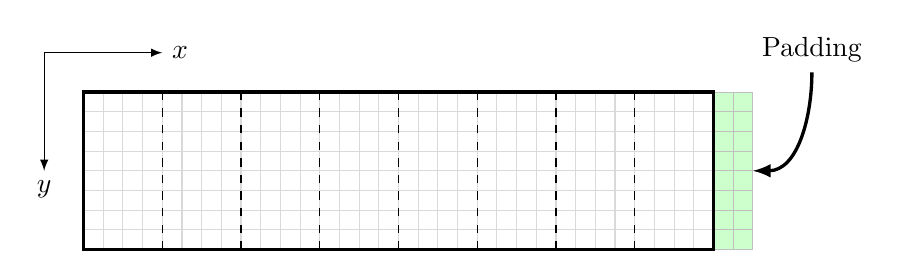
\begin{tikzpicture}[x=0.5cm,y=0.5cm]

\fill[green!20] (16,0) rectangle (17,4);
\draw[gray!30!white,step=0.5] (0,0) grid (16,4);
\draw[gray!50!white,step=0.5] (16,0) grid (17,4);
\draw[dashed,xstep=16/8,ystep=4] (0,0) grid (16,4);
\draw[very thick] (0,0) rectangle (16,4);

\coordinate (pad) at (17, 2);
\draw[-latex,very thick] (pad)+(1.5,+2.5) node[above] {Padding}
				to[out=-90,in=0] (pad);

\coordinate (O) at (-1, 5, 0);
\draw[-latex] (O) -- +(3, 0,  0) node [right] {$x$};
\draw[-latex] (O) -- +(0,  -3, 0) node [below] {$y$};
\end{tikzpicture}
\caption{A block divided in eight regions, each corresponding to a plasma chunk.  
Extra padding is added at the right for internal use in the FFTW library.}
\label{fig:block}
\end{figure}%}}}

A simplified representation of a block can be observed in the 
figure~\ref{fig:block}, where the X dimension of each field is contiguous in 
memory.  Notice the padding region in green, which is needed for the FFTW 
library to store intermediate values. The use of ghost elements is needed for 
communications and will be detailed in the chapter~\ref{ch:comm}. If we look at 
each cell $(x,y)$ in the block we find the four components $\rho(x,y)$, 
$\phi(x,y)$, $E_x(x,y)$ and $E_y(x,y)$.

\section{Simulation flow}

Before the main loop of the simulation begins, two previous iterations are 
required to prepare the simulation. The iteration counter is initially set to 
$-2$ to account for the extra steps.

\subsection{Allocation step}

After the creation of all MPI processes, the different structures to hold the 
data are allocated. Each process is assigned a block, with the corresponding 
fields and particles.

The fields are zeroed to begin the computation and the particles must be 
initialized following the user configuration. Each particle has an index which 
is used to let the user customize the particle attributes in case is required.  
Some initialization functions are provided, which place the particles following 
a random distribution or a specified pattern.

As the particles in a chunk are initialized, their position can set to any point 
in the physical space of the simulation, as no constraints are imposed for the 
initial placement. As a consequence, they need to be translated to the correct 
chunk before the simulation begins. We will refer to the initial movement of 
particles around the chunks as global communication, and is expected to last 
more than the typical communications once the simulation is running, as only 
local communications will be needed between neighbour chunks.

At soon as each particle is properly placed in the correct chunk, an initial 
computation of the charge density is done and the iteration counter is 
incremented.

\subsection{Rewind step}

The main loop begins with an special iteration that will only change the speed 
of the particles. The speed must be computed at half a time-step backwards in 
time, in order to use the leap-frog integrator as described in the 
section~\ref{sec:motion}. Once the iteration finishes, the main loop of can 
begin its normal execution with the iteration counter set to 0.

\subsection{Main loop}

The loop of the simulation performs four main steps:

\begin{itemize}
\item Accumulate charge density $\rho$ from the position of the particles.
\item Solve the field equation to get the electric field $\E$.
\item Interpolate the electric field $\E$ at particle positions.
\item Move the particles based on the computed force.
\end{itemize}

\section{Loop parallelization}

The four main steps of the simulation loop are parallelized following a common 
scheme: the block is partitioned in the same regions as the plasma chunks, which 
are processed in parallel.

\subsection{Charge accumulation}

%\begin{figure}[ht]%{{{
\begin{wrapfigure}{O}[2.7cm]{0.15\textwidth}
\centering
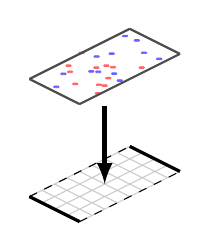
\begin{tikzpicture}[scale=0.85]
\begin{scope}[
		x=1cm,
		y=1cm,
		yshift=0,
		every node/.append style={
			yslant=0.5,xslant=-1},
		yslant=0.5,
		xslant=-1
	]
	\def\dx{0.0};
	% opacity to prevent graphical interference
	\draw[step=1.5/8, black!20!white, thin] (0,0-\dx) grid (6/4,6/8+\dx);
	%defining grids
	%\draw[step=1.5, black] (0,0) grid (6,6);
	\draw[xstep=1.5, ystep=0, black, very thick] (0,0-\dx) grid
		(6/4,6/8+\dx);
	\draw[dashed, xstep=6, ystep=1.5/2, black] (0,0) grid (6/4,6/8);

	\coordinate (b) at (1.5/2, 0.75/2);

\end{scope}
\begin{scope}[
		x=1cm,
		y=1cm,
		yshift=50,
		every node/.append style={
			yslant=0.5,xslant=-1},
		yslant=0.5,
		xslant=-1
	]
	\coordinate (c) at (1.5/2, 0.75/2);

	%\fill[fill=white,fill opacity=1.0] (0,0) rectangle (6,6);
	\begin{axis}[width=3cm,height=2.35cm,
						axis lines=none,
						%hide axis,
						xmin=-1, xmax=1,
						ymin=-1, ymax=1,
						inner frame sep=0,
				]
	\addplot [blue!60!white, only marks,
		mark=*, samples=12, mark size=0.75] (rand, rand);
	\addplot [red!60!white, only marks,
		mark=*, samples=12, mark size=0.75] (rand, rand);
	\end{axis}
	%\draw[step=1.5, black, thick] (0,0) grid (6,6);
	\draw[xstep=1.5, ystep=1.5/2, black!70!white, thick] (0,0) grid (6/4,6/8);
	%\draw[dashed,xstep=6, ystep=1.5, black, thick] (0,0) grid (6,6);


	\coordinate (O) at (1.5+0.5, 0.75+0.5);
\end{scope}

%\draw[-latex,very thick] (c)+(1,2) node[above]{Plasma chunk}
%				to[out=-90,in=90] (c);
%\draw[-latex,very thick,shorten >=3pt] (b)+(-1.5,-1) node[below]{Block}
%				to[out=90,in=180+45] (b);
\draw[-latex,ultra thick,shorten <=0.5cm]
	(c) to[out=-90,in=90] (b);
%	(c) to[out=-90,in=90]  node[midway,right]{Interpolation} (b);

\begin{scope}[
		y={(-1cm,0.5cm)},x={(1cm,0.5cm)}, z={(0cm,1cm)},
	]
%	\coordinate (O) at (-3, 3.5, 0);
%	\draw[-latex] (O) -- +(1, 0,  0) node [right] {$x$};
%	\draw[-latex] (O) -- +(0, -1, 0) node [right] {$y$};
%	\coordinate (O) at (-0.75, -0.75, 0);
%	\draw[-latex] (O) -- +(-1, 0,  0) node [left] {$y$};
%	\draw[-latex] (O) -- +(0, -1, 0) node [right] {$x$};
\end{scope}
\end{tikzpicture}
%\caption{Interpolation of the electric field $\E$ to the particles in a chunk.}
%\label{fig:interpolation-E}
\end{wrapfigure}
%\end{figure}%}}}
%
The interpolation process described in the equation~\ref{eq:charge-accumulation} 
is executed in parallel for all the particles of each chunk. The charge density 
field is being updated in parallel, which involves the four surrounding grid 
points of a particle, and it may happen that at the frontier of two chunks a 
concurrent access to the same element occurs.

To avoid a race condition with the next chunk, a dependency is added with the 
directive \texttt{commutative}, which allows the execution of the tasks in any 
order, but guarantees that a chunk can only be acessed by one task at a time. A 
detailed discussion on the directive can be found in the 
section~\ref{sec:exchange-x} with other alternatives to avoid a chain of 
dependencies in the case \texttt{inout} was used.

\begin{figure}[h]
\begin{lstlisting}[caption={Task to update $\rho$ field using the 
\texttt{commutative} directive}, captionpos=b]
for (i=0; i<plasma->nchunks; i++)
{
	c0 = &plasma->chunks[i];
	c1 = &plasma->chunks[(i + 1) % plasma->nchunks];
	#pragma oss task commutative(*c0, *c1) label(rho_update_0)
	rho_update(sim, i);
}
\end{lstlisting}
\end{figure}
% XXX Notice that we cannot have commutative in the next step or in the previous
% otherwise we can get ot of order execution in a chunk.

\subsection{Solve the fields}

Once the charge density is accumulated for each chunk, the electric potential 
can be computed by solving the Poisson equation (Eq.~\ref{eq:poisson}).  Using 
the MFT solver requires the computation of the Fourier transform of the charge 
density field, which has been purposely distributed among the Y dimension into 
blocks: The computation of the FFT can then be distributed into each process.

To parallelize the execution in each process, two mechanism are available in the 
FFTW library: pthreads and OpenMP. The multithreading design is based on the 
model of the \textit{parallel for}, where the total number of iterations are 
divided into parts that can be executed in parallel.
%
\begin{figure}[ht]%{{{
\begin{lstlisting}[
	%float,
	label={lst:openmp-for},
	caption={Parallel for with OpenMP used in the FFTW library.}]
#pragma omp parallel for private(d)
for (i = 0; i < nthr; ++i) {
	...
	proc(&d);
}
\end{lstlisting}
\end{figure}%}}}
%
In the listing~\ref{lst:openmp-for} the OpenMP parallelization method is shown, 
as used in the FFTW. With minor changes we can adapt the model to OmpSs-2, 
following the same approach. A task is created for each iteration and then we 
wait for the completion of all of them, ensuring all iterations of the loop have 
been executed, as can be seen in the listing~\ref{lst:ompss-for}. A comparative 
analysis of the different methods is provided in the chapter~\ref{ch:analysis}.
%
\begin{figure}[ht]%{{{
\begin{lstlisting}[
	%float,
	label={lst:ompss-for},
	caption={Parallel for with OmpSs-2 using tasks.}]
for (i = 0; i < nthr; ++i) {
	#pragma oss task private(d)
	{
		...
		proc(&d);
	}
}
#pragma oss taskwait
\end{lstlisting}
\end{figure}%}}}
%

Once we obtain the electric potential $\phi$ after the MFT algorithm, we can 
compute the electric field $\E$ in both directions $E_x$ and $E_y$. The 
operation can be fully parallelized in tasks by the division of the block in the 
same regions as the plasma chunks. It is not necessary that the same division is 
used, but has the advantage of simplify how the dependencies between plasma and 
fields are written.
%
\begin{figure}[ht]%{{{
\begin{lstlisting}[
label={lst:compute-E},
caption={Computation of E in parallel by chunks.}]
for(ic=0; ic<sim->plasma.nchunks; ic++)
{
	chunk = &sim->plasma.chunks[ic];
	#pragma oss task inout(*chunk) label(field_E_compute)
	field_E_compute(sim, chunk);
}
\end{lstlisting}
\end{figure}%}}}
%
The same division provided by the plasma chunks is used as a first approximation 
as shown in the listing~\ref{lst:compute-E}, but other number of regions are 
possible.

\subsection{Field interpolation}
%
%\begin{figure}[ht]%{{{
\begin{wrapfigure}{O}[2.5cm]{0.15\textwidth}
\centering
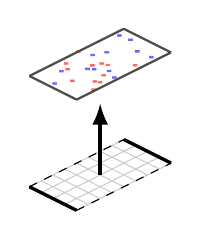
\begin{tikzpicture}[scale=0.8]
\begin{scope}[
		x=1cm,
		y=1cm,
		yshift=0,
		every node/.append style={
			yslant=0.5,xslant=-1},
		yslant=0.5,
		xslant=-1
	]
	\def\dx{0.0};
	% opacity to prevent graphical interference
	\draw[step=1.5/8, black!20!white, thin] (0,0-\dx) grid (6/4,6/8+\dx);
	%defining grids
	%\draw[step=1.5, black] (0,0) grid (6,6);
	\draw[xstep=1.5, ystep=0, black, very thick] (0,0-\dx) grid
		(6/4,6/8+\dx);
	\draw[dashed, xstep=6, ystep=1.5/2, black] (0,0) grid (6/4,6/8);

	\coordinate (b) at (1.5/2, 0.75/2);

\end{scope}
\begin{scope}[
		x=1cm,
		y=1cm,
		yshift=50,
		every node/.append style={
			yslant=0.5,xslant=-1},
		yslant=0.5,
		xslant=-1
	]
	\coordinate (c) at (1.5/2, 0.75/2);

	%\fill[fill=white,fill opacity=1.0] (0,0) rectangle (6,6);
	\begin{axis}[width=3cm,height=2.35cm,
						axis lines=none,
						%hide axis,
						xmin=-1, xmax=1,
						ymin=-1, ymax=1,
						inner frame sep=0,
				]
	\addplot [blue!60!white, only marks,
		mark=*, samples=12, mark size=0.75] (rand, rand);
	\addplot [red!60!white, only marks,
		mark=*, samples=12, mark size=0.75] (rand, rand);
	\end{axis}
	%\draw[step=1.5, black, thick] (0,0) grid (6,6);
	\draw[xstep=1.5, ystep=1.5/2, black!70!white, thick] (0,0) grid (6/4,6/8);
	%\draw[dashed,xstep=6, ystep=1.5, black, thick] (0,0) grid (6,6);


	\coordinate (O) at (1.5+0.5, 0.75+0.5);
\end{scope}

%\draw[-latex,very thick] (c)+(1,2) node[above]{Plasma chunk}
%				to[out=-90,in=90] (c);
%\draw[-latex,very thick,shorten >=3pt] (b)+(-1.5,-1) node[below]{Block}
%				to[out=90,in=180+45] (b);
\draw[-latex,ultra thick,shorten >=0.5cm]
	(b) to[out=90,in=-90] (c);
%	(b) to[out=90,in=-90]  node[midway,right]{Interpolation} (c);

\begin{scope}[
		y={(-1cm,0.5cm)},x={(1cm,0.5cm)}, z={(0cm,1cm)},
	]
%	\coordinate (O) at (-3, 3.5, 0);
%	\draw[-latex] (O) -- +(1, 0,  0) node [right] {$x$};
%	\draw[-latex] (O) -- +(0, -1, 0) node [right] {$y$};
%	\coordinate (O) at (-0.75, -0.75, 0);
%	\draw[-latex] (O) -- +(-1, 0,  0) node [left] {$y$};
%	\draw[-latex] (O) -- +(0, -1, 0) node [right] {$x$};
\end{scope}
\end{tikzpicture}
%\caption{Interpolation of the electric field $\E$ to the particles in a chunk.}
%\label{fig:interpolation-E}
\end{wrapfigure}
%\end{figure}%}}}
%
Once the electric field of a chunk is ready, the value is interpolated at the 
particle locations. The force will be obtained in the next step from the 
interpolated electric field in each particle.

Each chunk can be processed independently by one task, but a \texttt{inout} 
dependency must be added to ensure the order of execution of a chunk is done 
after the electric field is computed, as observed in the 
listing~\ref{lst:interpolate-E}.
%
\begin{figure}[ht]%{{{
\begin{lstlisting}[
label={lst:interpolate-E},
caption={Interpolation of the electric field $\E$ at particle position.}]
for(i=0; i<sim->plasma.nchunks; i++)
{
	chunk = &sim->plasma.chunks[i];
	#pragma oss task inout(*chunk) label(chunk_E)
	{
		for(is=0; is<chunk->nspecies; is++)
		{
			particle_set_E(sim, chunk, is);
		}
	}
}
\end{lstlisting}
\end{figure}%}}}
%
\subsection{Particle mover}

The force acting on each particle is obtained as described in the 
equation~\ref{eq:force}, as the combination of the electric and magnetic forces.  
The electric term is computed from the interpolated electric field at the 
particle locations and each chunk can begin the process as soon as the 
interpolation process has finished.

A task is created for each chunk, and the particles are moved accordingly to the 
obtained force. The Boris integrator described in the section~\ref{sec:boris} is 
used to accurately position the particles. An \texttt{inout} dependency is added 
to each chunk to guarantee the order of execution: after the electric field is 
interpolated in the particles, as shown in the listing~\ref{lst:particle-mover}.
%
\begin{figure}[ht]%{{{
\begin{lstlisting}[
label={lst:particle-mover},
caption={Movement of particles based on the interpolated field $\E$.}]
for(i=0; i<sim->plasma.nchunks; i++)
{
	chunk = &sim->plasma.chunks[i];
	#pragma oss task inout(*chunk) label(chunk_x_update)
	{
		for(is=0; is<chunk->nspecies; is++)
		{
			particle_x_update(sim, chunk, is);
		}
	}
}
\end{lstlisting}
\end{figure}%}}}

\chapter{Communication}

Different communications are detailed in this chapter, such as particle and 
frontier communications.

\section{Particle communication}

When the particles are moved, due to the interaction with the electric field and 
the magnetic field, their position can exceed the boundaries of the chunk where 
they reside. After updating the position of each particle, the ones that exceed 
the chunk must be translated to the correct one. The process of particle 
communication is done in two stages: first the particles are moved in the X 
dimension, then in the Y. Several steps are required in each stage.

\subsection{Exchange in X}
%TODO Place figure to describe the movement
All chunks in the X dimension reside in one MPI process, so the exchange of 
particles can be done by shared memory. Care must be taken to avoid concurrent 
writes in the same chunk by different tasks. The proposed solution avoids the 
problem by using temporal queues in each chunk. The process can be described in 
the following steps:
%
\begin{enumerate}
\item \texttt{collect\_particles\_x}: Out of bound particles in the X direction 
are extracted from the chunk and placed in the correct target chunk queue for 
local exchange.
\item \texttt{exchange\_particles\_x}: Each chunk looks for particles in the 
neighbour chunks target queues and moves them to itself.
\end{enumerate}
%
Usually only two target queues are required for each chunk, as the particles can 
only move one chunk per iteration. However, in the initial iteration after the 
initialization of the particle positions, they can move to any other chunk, and 
the process is subsequently more computationally expensive. We will only focus 
in the general case involving only the two neighbours, as the initialization 
iteration can be disregarded when comparing the time against the whole 
simulation.

% TODO:Should we split this details in another section/chapter involving only
% tasks and TAMPI?
Each step can be implemented using tasks with dependencies, in order to exploit 
local parallelism. One task collects the particles out of the chunk in the 
corresponding queues, so it needs to access only the current chunk.
%
\begin{lstlisting}
for(i = 0; i < plasma->nchunks; i++)
{
	chunk = &plasma->chunks[i];
	/* Place each particle outside a chunk in the X dimension, in
	 * the lout list */
	#pragma oss task inout(*chunk) label(collect_particles_x)
	for(is = 0; is < sim->nspecies; is++)
	{
		collect_particles_x(sim, chunk, is, global_exchange);
	}
}
\end{lstlisting}
%
The exchange process can now run in parallel, but the task can only run if the 
collecting process has finished in the neighbour chunks, as otherwise the queues 
are still being written. The dependencies can be placed in all involved chunks.
%
\begin{lstlisting}
for (i = 0; i < plasma->nchunks; i++)
{
	chunk = &plasma->chunks[i];
	...

	#pragma oss task inout(*chunk) \
@          inout(*prev_chunk) inout(*next_chunk) \
@          label(exchange_particles_x)
	{
		/* Only the two neighbours are needed */
		concat_particles(chunk, prev_chunk);
		concat_particles(chunk, next_chunk);
	}
}
\end{lstlisting}
%
Notice that in the first iteration the exchange step must wait for all the 
collecting tasks to finish, as the particles can be moved to any chunk, and thus 
we expect to see a slower iteration than the rest of the simulation. In the 
following steps, only the neighbours at $i-1$, $i$ and $i+1$ are required to 
finish the exchange process.

\begin{figure}[h]
	\centering
	\subfloat[Chain of dependencies observed]{
		\includegraphics[width=0.7\textwidth]{chain}
		\label{fig:chain}
	}
	\\
	\subfloat[The chain has been corrected]{
		\includegraphics[width=0.7\textwidth]{no-chain}
		\label{fig:no-chain}
	}
	\caption{Comparison of two \texttt{paraver} traces using coloring tasks for 
	communication.}
\end{figure}
%
However, there is a problem with the previous loop: as we create the 
dependencies with the next chunk before the next task is created, we are 
building a chain. Using \texttt{paraver} we can clearly see the chain in the 
trace graph, shown in the figure~\ref{fig:chain}, where no task can run in 
parallel until the previous one finishes.  One solution to alleviate this 
problem is the use of colors, where the loops creates all tasks of the same 
color first, then the ones with the next color and so on.  With three colors we 
ensure that the two tasks of the same color can run in parallel without 
concurrent access to the same chunk.
%
\begin{lstlisting}
max_color = 3;

for(color = 0; color < max_color; color++)
{
	/* Use coloring to prevent a chain of dependencies */
	for(i = color; i < plasma->nchunks; i+=max_color)
	{
		chunk = &plasma->chunks[i];
		...

		#pragma oss task inout(*chunk) \
	@              inout(*prev_chunk) inout(*next_chunk) \
	@              label(collect_local_particles)
		{
			/* Only the two neighbours are needed */
			concat_particles(chunk, prev_chunk);
			concat_particles(chunk, next_chunk);
		}
	}
}
\end{lstlisting}
%
In the figure~\ref{fig:no-chain} we can now observe how the chain has 
disappeared, and the holes are now fully covered by tasks running in parallel.

Once all exchange tasks are completed, all particles are now placed in the 
correct chunk in the X dimension, and only the Y movement is left.

\subsection{Exchange in Y}
%TODO Place figure to describe the movement
Once the particles are placed in the correct chunk in the X dimension, the 
displacement to the correct chunk in the Y dimension involves sending the 
particles to another MPI process. The steps can be resumed as
%
\begin{enumerate}
\item \texttt{collect\_particles\_y}: Place each particle out of the chunk 
bounds in a queue (one for each target destination).
\item \texttt{pack\_particles\_y}: Pack the particles to be sent to the 
neighbour chunk in a message.
\item \texttt{send\_particles\_y}: Send the packed particles to each neighbour.
\item \texttt{recv\_particles\_y}: Receive the message with the packed 
particles.
\item \texttt{unpack\_particles\_y}: Unpack the particle message and place the 
particles in the chunk.
\end{enumerate}
%
\begin{figure}
\centering
\includegraphics[width=\textwidth]{comm-particles.pdf}
\caption{Graph of task and dependencies of particle communication in 
Y}
\label{fig:comm_y}
\end{figure}
%
Similarly as for the horizontal direction, the particles exceeding the limits of 
each chunk in the Y dimension are placed in a queue.  Once the particles are 
identified within a chunk, they are packed in a message in a contiguous memory 
region. This buffer is then sent using \texttt{MPI\_Send} to the neighbour 
process.

The reception process works in the opposite order: each chunk receives the 
communication of the neighbour chunks in the vertical direction. Once a message 
is received is unpacked and the particles are added to the chunk. In the 
diagram~\ref{fig:comm_y} the dependencies of each step are shown in a graph.

Notice that all the MPI communication is independent of the neighbour chunks in 
the horizontal direction, and can be fully parallelized. Some constraints must 
be added to coordinate the vertical communications to guarantee that no 
simultaneous writes occur in the same chunk.

\begin{lstlisting}
for(i = 0; i < plasma->nchunks; i++)
{
	chunk = &plasma->chunks[i];

	/* Collect particles in a queue that need to change chunk */
	#pragma oss task inout(*chunk) label(collect_particles_y)
	for(is = 0; is < sim->nspecies; is++)
	{
		collect_particles_y(sim, chunk, is, global_exchange);
	}

	/* Prepare the packet to be sent to the neighbour */
	#pragma oss task inout(*chunk) label(pack_particles_y)
	pack_particles_y(sim, chunk, i, global_exchange);

	/* Finally send the packet */
	#pragma oss task in(*chunk) label(send_particles_y_y)
	send_particles_y(sim, chunk, i, global_exchange);

	/* We cannot create here a task as we don't know the dependencies
	 * when using MPI */
	recv_particles_y(sim, chunk, global_exchange);
}
\end{lstlisting}

%\chapter{Analysis}


%\section{Analyze time distribution}

In order to reduce the amount of CPU time involved in each step of the 
simulation, the best strategy is to reduce the time spent in the most time 
consuming part.

The CPU time involved in each part of the simulation may depend on various 
factors, such as the number of grid points, the number of particles or the 
boundary conditions. As an example, consider a simulation with a large number of 
grid points, with few particles---the computation of the electric field 
(\texttt{field\_E}) will dominate the simulation time, as shown in the figure 
\ref{fig:cm-big-grid}. In a case of a large number of particles and a smaller 
grid, the particle interpolation (\texttt{particle\_E}) dominates the whole 
execution as seen in the figure \ref{fig:cm-lots-particles}.

\begin{figure}[h]
	\centering
	\subfloat[1024 particles, 512x512 grid points]{
		\includegraphics[width=\linewidth]{callmap-grid512x512-n1024.png}
		\label{fig:cm-big-grid}
	}
	\\
	\subfloat[10240 particles, 64x64 grid points]{
		\includegraphics[width=\linewidth]{callmap-grid64x64-n10240.png}
		\label{fig:cm-lots-particles}
	}
	\caption{Comparison of the time spent in each function at two different 
	simulations.}
\end{figure}

In order to optimize the general use case, different inputs will be tested and 
the main simulation steps will be characterized. Furthermore, different 
algorithms or methods may be used to improve the speed. As an example, the LU 
algorithm is compared with the spectral method MFT.

\section{Analysis with varying inputs}


\chapter{Analysis of performance}
\label{ch:analysis}

\pgfplotsset{
	every axis/.append style={
		line width=.5 pt,
		tick style={line width=.6pt},
		label style={font=\footnotesize},
		tick label style={font=\footnotesize},
	}
}

The time of the simulation will be used to characterize the performance when 
several parameters are changed. The time is measured using the wall clock, and 
refers to the \textit{time per iteration}. Sometimes the different stages of the 
simulator will be measured as well, to give more insight in the distribution of 
the time. Notice that each process may start or end a iteration at different 
times, by in the long run all processes must be synchronized. The measurements 
will take place only in the first process (with rank zero).

At each iteration various factors may affect the iteration time and introduce a 
random delay. We will model the simulation time as $t = \hat t + e_t$, where the 
true simulation time $\hat t$ is unknown but constant between iterations, and 
the error $e_t$ is a random variable with zero mean and unknown but finite 
variance $\sigma^2$.  Additionally, we will assume that the error $e_t$ is 
independent and identically distributed in each iteration of the same 
configuration and that follows a normal distribution.

We can then consider the sequence of measured times $T = t_1,\ldots,t_n$ as 
independent random variables from a common distribution with an unknown mean 
$\hat t$ and finite standard deviation $\sigma$. The sample mean $\overline T$ 
can be approximated with a certain degree of confidence by a process of 
sampling. The standard error of the mean (SEM) will be used to get a confidence 
interval in which we can ensure the true mean is located. The standard error of 
the mean is defined as:
%
\begin{equation}
\epsilon = \frac{\sigma}{\sqrt{n}}
\end{equation}
%
As the standard deviation $\sigma$ is unknown, following the assumption that the 
error follows a normal distribution, we can use the student distribution to get 
the standard error using the standard deviation of the sample $s$
%
\begin{equation}
\epsilon = Z_\alpha\frac{s}{\sqrt{n}}
\end{equation}
%
With a significance level $\alpha=0.05$ we get from the t-student distribution 
the value $Z=1.96$, and we can obtain the confidence interval $\overline T \pm 
\epsilon$ where we can ensure the true mean is located with a probability of 
95\% \cite{ross}. By setting the relative error $\delta = \epsilon / \overline 
T$ to be lower than 1\%, we obtain the limit error $\epsilon_0$ to be 
$\epsilon_0 = 
0.01 \overline T$.
%
Then, if we stop the simulation process when the standard error of the mean is 
below $\epsilon_0$
%
\begin{equation}
\epsilon = Z_\alpha\frac{s}{\sqrt{n}} < 0.01 \, \overline T
\end{equation}
%
We can ensure that (a) with probability 0.95 the true mean $\hat t$ is located 
in the interval $\overline T \pm \epsilon$, and (b) the relative error of the 
mean $\delta$ is lower than 1\%.

The process of simulation will run for at least a minimum of 30 iterations. Then 
it will continue until the relative error is below 1\%, or the simulation time 
exceeds 30 minutes.
%
All experiments were run in the MareNostrum 4 supercomputer \cite{mn4}, using 
Intel MPI and the Intel \texttt{icc} compiler with the following modules:
%\setlength{\columnsep}{-2.1in}
\begin{multicols}{3}
\begin{itemize}
\item intel/2017.4
\item fftw/3.3.6
\item tampi/1.0
\item impi/2017.4
\item ompss-2/2019.06
\item extrae/3.7.0
\end{itemize}
\end{multicols}

%
%\vspace{1em}
%\todo[inline]{Use error bars to denote CI at 95\% not std?}

\section{Performance model}

Consider the real time of the simulation $\hat t(c)$ to be a function of a 
specific configuration $c$. There are a lot of parameters that may be changed 
and have some influence in the time per iteration, but we will focus only on the 
following ones.
%
\begin{itemize}
\item $N_p$: Number of total particles.
\item $N_g$: Number of total grid points.
\item $N_c$: Number of plasma chunks.
\item $P$: Number of total MPI processes.
\item $C$: Number of total cores (the sum of cores in all processes).
\item $A$: Whether TAMPI ($A = 1$) or MPI ($A=0$) is being used.
\end{itemize}
%
A configuration is then completely specified as the tuple $c = (N_p, N_g, N_c, 
P, C, A)$. The space of states of configurations possible is bigger than the 
available time for experimentation, so we must choose a partial group which can 
reveal interesting information of the effect in the iteration time.
%
\subsection{Number of particles}

The number of particles $N_p$ is one of the main parameters that affect the
running time of each iteration as it can be observed from the simulation process 
that at least a complexity in $O(N_p)$ is expected---we need to cycle through 
each particle at every iteration. To get an accurate relation, an experiment is 
run sweeping from \num{2e6} to \num{4e7} particles, with 32 cores and only one 
process. The number of grid points is kept low at $1024^2$ in order to avoid 
interference from the solver. We see in the figure~\ref{fig:particles-32cpus} 
how the time scales linearly with the number of particles, and the residuals of 
the linear regression. With a determination coefficient of $R^2 = 0.99981$, we 
can estimate a time per particle of \SI{51.4}{\micro\second} with 32 cores.

\begin{figure}[h]%{{{
	\centering
	\begin{tikzpicture}
	\begin{axis}[
		width=0.5\textwidth,
		xlabel=Particles $N_p$,
		ylabel=Time per iteration (s),
		no markers,
		%grid=major,
	]
	\addplot [only marks,scatter,error bars/y dir=both, error bars/y explicit] 
	table [
		x index = {0},
		y index = {3},
		y error index={4},
		col sep=space] {perf/particles/csv/time.csv};
	\addplot [red] table [col sep=space] {perf/particles/csv/regression.csv};
	\end{axis}
	\end{tikzpicture}
	\begin{tikzpicture}
	\begin{axis} [
		yticklabel pos=right,
		xlabel=Particles $N_p$,
		ylabel=Residuals (s),
		width=0.5\textwidth,
		%grid=major,
	]
	\addplot [
		only marks,
		error bars/y dir=both,
		error bars/y explicit,
	] table [
		x index = {0},
		y index = {2},
		y error index = {3},
		col sep=space] {perf/particles/csv/regression.csv};
	\draw[
		ultra thin,
		black!30!white
	] (axis cs:\pgfkeysvalueof{/pgfplots/xmin},0) --
			(axis cs:\pgfkeysvalueof{/pgfplots/xmax},0);
	\end{axis}
	\end{tikzpicture}
	\caption{The number of particles $N_p$ is increased and the time per iteration 
	$t$ is measured. A linear regression fit is shown, with the residuals at the 
	left. Using one process and 32 CPUs MPI communications are not needed.  
	Configuration used ($N_p=\num{2e6}\text{ to }\num{4e7}$, $N_g = 1024^2$, 
	$N_c=128$, $P=1$, $C=32$, $A=1$)}
	\label{fig:particles-32cpus}
\end{figure}%}}}

\subsection{Number of grid points}

The MFT solver uses the FFTW library to perform the FFT and solve the field 
equation in each iteration, with an expected worst time complexity in $O(N_g 
\log N_g)$. An experiment with varying number of grid points from $2048^2$ to 
$8192^2$ is designed to observe the grow in time.
%
\begin{figure}[h]%{{{
	\centering
	\begin{tikzpicture}
	\begin{axis} [
			no markers,
			grid=major,
			xlabel=Grid points $N_g$,
			ylabel=Time per iteration (s),
			width=0.5\textwidth]
		\addplot [scatter,only marks,error bars/y dir=both, error bars/y explicit] 
		table [
			x index = {0},
			y index = {3},
			y error index={4},
			col sep=space] {perf/gridpoints/time.csv};
		\addplot [red] table [col sep=space] {perf/gridpoints/csv/regression.csv};
	\end{axis}
	\end{tikzpicture}
	\begin{tikzpicture}
	\begin{axis} [
		yticklabel pos=right,
		xlabel=Particles $N_p$,
		ylabel=Residuals (s),
		width=0.5\textwidth,
		%grid=major,
	]
	\addplot [
		only marks,
		error bars/y dir=both,
		error bars/y explicit,
	] table [
		x index = {0},
		y index = {2},
		y error index = {3},
		col sep=space] {perf/gridpoints/csv/regression.csv};
	\draw[
		ultra thin,
		black!30!white
	] (axis cs:\pgfkeysvalueof{/pgfplots/xmin},0) --
			(axis cs:\pgfkeysvalueof{/pgfplots/xmax},0);
	\end{axis}
	\end{tikzpicture}
	\caption{The effect of the variables $N_p$ and $N_g$ to the time per 
	iteration. Using one process and 32 CPUs (MPI communications are not needed).}
	\label{fig:gridpoints-32cpus}
\end{figure}%}}}
%
In the figure~\ref{fig:gridpoints-32cpus} it can be seen how the time grows with 
the number of grid points following the complexity $O(N_g \log N_g)$, but the 
variance is much bigger than with the number of particles. Notice that the 
dispersion is not due to random variations in the execution time, as the 
standard deviation for each point is lower than its dispersion from the common 
distribution. The FFTW uses an algorithm which benefits from sizes that can be 
decomposed into the product of small multiples ($2^a \cdot 3^b\cdot 5^c\cdot 
7^d\,\ldots$).  However the number of points in the X axis must be divisible by 
the number of plasma chunks, and some of the sizes tested had large primes in 
their decomposition.
%
%\todo[inline]{Regenerate figure with appropriate sizes and check the dispersion 
%decreases.}
%

\section{Solver multithreading scalability}

The simulator is designed to scale with the number of particles when the number 
of cores or MPI processes are incremented---each chunk can be computed in 
parallel both in the X and Y axis. But when the number of grid points is 
incremented, the FFT solver must scale both in the number of CPUs and processes.  

The space in Y is divided into equally sized blocks, which are assigned into MPI 
processes, following the parallelization design of the FFTW. Additionally the 
library offers two parallelization implementations for multithreading: Using 
OpenMP and POSIX threads (pthreads).  OpenMP is not compatible with OmpSs-2 as 
we have one runtime already running so the pthread implementation was tested.
%
\begin{figure}[h]%{{{
	\centering
		\begin{tikzpicture}
		\begin{axis} [
			legend pos=north west,
			xmode=log,
			log basis x=2,
			xticklabels={0,1,2,4,8,16,32},
			grid=major,
			xlabel=Number of CPUs,
			ylabel=Time per iteration (s),
			width=10cm,
			height=6cm,
			]
		\addplot+ [error bars/y dir=both, error bars/y explicit] table [
			x index = {0},
			y index = {3},
			y error index={4},
			col sep=space] {perf/fftw-sequential/time.csv};
		\addlegendentry{Single thread}
		\addplot+ [error bars/y dir=both, error bars/y explicit] table [
			x index = {0},
			y index = {3},
			y error index={4},
			col sep=space] {perf/fftw-threads/time.csv};
		\addlegendentry{Multithread}
		\end{axis}
		\end{tikzpicture}
	\caption{The number of CPUs is increased with only one process: the solver 
	cannot scale and the time per iteration increases. Configuration used: $N_p = 
	\num{5e5}$, $N_g=8192\times8192$.}
	\label{fig:fftw-time}
\end{figure}%}}}
%
Unfortunately, the FFTW library doesn't show a good speedup, in fact worsens the 
time per iteration when adding more threads with the configurations tested. In 
the figure~\ref{fig:fftw-time} it can be shown how the time grows as the number 
of CPUs increases.
%
The FFTW documentation warns about this problem, claiming that it can only 
improve the time with large enough matrices:
%
\begin{displayquote}
{\sl ``A shared-memory machine is one in which all CPUs can directly access the 
same main memory, and such machines are now common due to the ubiquity of 
multi-core CPUs. FFTW’s multi-threading support allows you to utilize these 
additional CPUs transparently from a single program. However, this does not 
necessarily translate into performance gains---when multiple threads/CPUs are 
employed, there is an overhead required for synchronization that may outweigh 
the computational parallelism. Therefore, you can only benefit from threads if 
your problem is sufficiently large.''}---FFTW Online manual \cite{FFTW-manual}.
\end{displayquote}
%
However, larger matrices are not useful to get more precise results, as usually 
is the increase in the number of particles what provides more information of the 
behavior of plasma in complex simulations.

\begin{figure}[h]%{{{
	\centering
	\includegraphics[width=0.95\linewidth]{fftw-ompss2.png}
	\caption{Tasks created inside the FFTW when using OmpSs-2: Up to 450 tasks are 
	created in rapid succession, with only 4 CPUs and 2 processes.}
	\label{fig:fftw-ompss2}
\end{figure}%}}}

In order to avoid a scalability problem, another approach was tested: Adding 
support for OmpSs-2~in the FFTW to enable multithreading, following the same 
structure as OpenMP. The results obtained were similar as with the pthread case, 
but more insight was gained in how the task were being created. In the 
figure~\ref{fig:fftw-ompss2} it can be shown that the overhead added by the 
large amount of created tasks outweight any benefit that could be gained by 
multithreading.

\begin{figure}[h]%{{{
	\centering
		\begin{tikzpicture}
		\begin{axis} [
			legend pos=outer north east,
			xmode=log,
			log basis x=2,
			xticklabels={0,1,2,4,8,16},
%			xticklabel style={
%			/pgf/number format/precision=3,
%			/pgf/number format/fixed},
			grid=major,
			xlabel=Number of CPUs per process,
			ylabel=Time per iteration (s),
			width=0.5\textwidth]
		\addplot [ybar stacked, fill=red!30!white] table [
			x index = {0},
			y index = {10},
			col sep=space] {perf/constant-cpus/time.csv};
		\addlegendentry{Solver}
		\addplot [ybar stacked, fill=blue!30!white] table [
			x index = {0},
			y index = {11},
			col sep=space] {perf/constant-cpus/time.csv};
		\addlegendentry{Particles}
		\addplot [only marks,error bars/y dir=both, error bars/y explicit] table [
			x index = {0},
			y index = {5},
			y error index={6},
			col sep=space] {perf/constant-cpus/time.csv};
		\addlegendentry{Total}
		\end{axis}
		\end{tikzpicture}
	\caption{The number of CPUs per process is incremented while reducing the 
	number of processes (the total number of CPUs is set to 32 and is kept 
	constant).  The time per iteration is measured, which leads to a 
	characteristic U shape.}
	\label{fig:fftw-u}
\end{figure}%}}}

We can mitigate the problem by increasing the number of MPI processes. In order 
to evaluate which ratio of processes and CPUs yields the best performance 
several configurations are tested. With a fixed number of maximum CPUs available 
set to 32, we increase the number of processes while we reduce the CPUs per 
process as shown in the figure~\ref{fig:fftw-u}.

As the ratio of CPUs per process in incremented, while decreasing the number of 
processes, the solver begins to increase the execution time. Meanwhile, the part 
of the simulation involving the particles, which can be fully parallelized shows 
a decrease in time. The optimal ratio for the chosen configuration seems to be 
around 4 CPUs per process.

%\begin{figure}[h]{{{
%	\centering
%		\begin{tikzpicture}
%		\begin{axis} [
%			baseline,
%			xmode=log,
%			log basis x=2,
%			xticklabels={0,1,2,4,8,16},
%%			xticklabel style={
%%			/pgf/number format/precision=3,
%%			/pgf/number format/fixed},
%			grid=major,
%			xlabel=Number of CPUs per process,
%			ylabel=Time per iteration (s),
%			ymax=6,
%			width=0.5\textwidth,
%			height=10cm,
%			]
%		\foreach \Nc in {32,64,128,256,512} {
%			\edef\temp{\noexpand\addlegendentry{$N_c = \Nc$}}
%			\addplot+ table [
%				x = P,
%				y = mean,
%				y error = {rel-err},
%				col sep=tab] {csv/mpi-scaling/Nc\Nc};
%			%\temp
%		}
%		\end{axis}
%		\end{tikzpicture}
%		\hspace{0.15cm}
%		\begin{tikzpicture}
%		\begin{axis} [
%			baseline,
%			xmode=log,
%			log basis x=2,
%			xticklabels={0,1,2,4,8,16},
%%			xticklabel style={
%%			/pgf/number format/precision=3,
%%			/pgf/number format/fixed},
%			grid=major,
%			xlabel=Number of CPUs per process,
%			ylabel=Time per iteration (s),
%			height=10cm,
%			width=0.5\textwidth]
%		\foreach \Nc in {32,64,128,256,512} {
%			\edef\temp{\noexpand\addlegendentry{$N_c = \Nc$}}
%			\addplot+ table [
%				x = P,
%				y = mean,
%				y error = {rel-err},
%				col sep=tab] {csv/tampi-scaling/Nc\Nc};
%			\temp
%		}
%		\end{axis}
%		\end{tikzpicture}
%	\caption{The number of CPUs per process is incremented while reducing the 
%	number of processes (the total number of CPUs is set to 32 and is kept 
%	constant).  The time per iteration is measured, which leads to a 
%	characteristic U shape.}
%\end{figure}}}}

\section{TAMPI}

The two modes of communication are compared with different configurations, in 
order to evaluate the effect in the overall performance of the simulation. The 
chunk size $N_c$ determines the number of messages sent per process and is 
tested from 32 to 512.
%
\begin{figure}%{{{
\centering
\begin{tikzpicture}
	\begin{groupplot}[
		group style={
			columns=2,
%			rows=2,
			horizontal sep=0.5cm,
			ylabels at=edge left,
			yticklabels at=edge left,
		},
		xmode=log,
		log basis x=2,
%		xticklabels={0,1,2,4,8,16},
		grid=major,
		xmin=0,
		ymin=0,
		xlabel=Number of processes,
		ylabel=Time per iteration (s),
		height=10cm,
		width=7cm,
		/tikz/font=\small]
	\nextgroupplot[
		ymax=6,
		title={MPI},
%		error bars/y dir=both,
%		error bars/y explicit
	]
	\foreach \Nc in {32,64,128,256,512} {
		\edef\temp{\noexpand\addlegendentry{$N_c = \Nc$}}
		\addplot+ table [
			x = P,
			y = mean,
			y error = {rel-err},
			col sep=tab] {perf/mpi-scaling/csv/Nc\Nc};
		%\temp
	}
% Using inout is slightly slower than commutative
%	\nextgroupplot[ymax=6,title={MPI with inout}]
%	\foreach \Nc in {32,64,128,256,512} {
%		\edef\temp{\noexpand\addlegendentry{$N_c = \Nc$}}
%		\addplot+ table [
%			x = P,
%			y = mean,
%			y error = {rel-err},
%			col sep=tab] {csv/mpi-inout-scaling/Nc\Nc};
%		%\temp
%	}
	\nextgroupplot[
		ymax=6,
		title={TAMPI},
%		error bars/y dir=both,
%		error bars/y explicit
	]
	\foreach \Nc in {32,64,128,256,512} {
		\edef\temp{\noexpand\addlegendentry{$N_c = \Nc$}}
		\addplot+ table [
			x = P,
			y = mean,
			y error = {rel-err},
			col sep=tab] {perf/tampi-scaling/csv/Nc\Nc};
		\temp
	}
	\end{groupplot}
\end{tikzpicture}
\caption{Comparison of MPI and TAMPI}
\label{fig:TAMPI}
\end{figure}%}}}
%
In the figure~\ref{fig:TAMPI} it can be seen how the time is drastically reduced 
when TAMPI is enabled. The performance difference is lower when the number of 
processes increases, but is very significant with few processes. Notice the 
control case with only one process were no MPI nor TAMPI communication is needed 
(shared memory is used to exchange information between tasks).

It is also noted with MPI a saturation point with 512 chunks per process, where 
the time does not improve with more processes. Different versions of OpenMPI 
(3.1.1, 4.0.0 and 4.0.1) were also tested, and there was a extreme delay of more 
than one order of magnitude with respect to the mean time per iteration with low 
probability of occurrence, and the causes are yet unknown. The same problem was 
never observed with Intel MPI, but further investigation is needed to isolate 
the issue and conclude that is due to OpenMPI.

In the following experiments, we will always enable TAMPI for the 
communications, unless explicitly stated otherwise.

\section{Scalability}

In order to evaluate the simulator in terms of scalability the two main metrics 
are initially measured:
\begin{enumerate}
\item \textbf{Strong scalability}: The same configuration of problem is repeated 
with increasing number of computing elements.
\item \textbf{Weak scalability}: The number of computing elements is increased, 
while the amount of work assigned to each one is kept constant by changing the 
problem configuration.
\end{enumerate}
%
%
\begin{figure}[ht]%{{{
\centering
\begin{tikzpicture}
	\begin{axis}[
		xmode=log,
		log basis x=2,
		xticklabels={0,1,2,4,8,16,32},
		grid=major,
		xmin=0,
		ymin=0,
		xlabel=Number of nodes,
		ylabel=Speedup,
		height=8cm,
		width=0.5\textwidth,
		/tikz/font=\small]
		\addplot+ table [
			x = P,
			y = speedup,
			col sep=tab] {perf/strong-scaling-fixed/csv/time.csv};
	\end{axis}
\end{tikzpicture}
\begin{tikzpicture}
	\begin{axis}[
		xmode=log,
		log basis x=2,
		xticklabels={0,1,2,4,8,16,32},
		grid=major,
		xmin=0,
		ymin=0,
		xlabel=Number of nodes,
		ylabel=Efficiency,
		height=8cm,
		width=0.5\textwidth,
		/tikz/font=\small]
		\addplot+ table [
			x = P,
			y = efficiency,
			col sep=tab] {perf/strong-scaling-fixed/csv/time.csv};
	\end{axis}
\end{tikzpicture}
	\caption{Strong scaling with configuration: $N_p = \num{1e8}$, $N_g = 2048^2$,
	$N_c = 128$, one process per node, using each 48 cores.}
	\label{fig:strong-scaling}
\end{figure}%}}}
%
For the strong scalability, a fixed configuration of $N_p = \num{1e8}$ 
particles, $N_g=2048^2$ grid points and $N_c=128$ chunks is used to run the 
simulator with increasing number of computing nodes. Each node runs with 48 
cores---all the available CPUs of the machine. In the 
figure~\ref{fig:strong-scaling} the speedup and the efficiency are shown.
The rapid decay of efficiency is to be expected, as the solver cannot exploit 
the full 48 cores and only one is used when solving the FFT. We can obtain more 
information of the scalability of the simulator without the solver by disabling 
it---the physical result of the simulation will be non-sense, but the same 
stages of the simulator will be executed as if the solver was enabled. We see in 
the figure~\ref{fig:strong-scaling-without-solver} how the efficiency now 
improves substantially, and indicates that the solver is acting as a bottle neck 
which leads to a significant reduction in scalability.
%
\begin{figure}[ht]%{{{
\centering
\begin{tikzpicture}
	\begin{axis}[
		xmode=log,
		log basis x=2,
		xticklabels={0,1,2,4,8,16,32},
		grid=major,
		xmin=0,
		ymin=0,
		xlabel=Number of nodes,
		ylabel=Speedup,
		height=8cm,
		width=0.5\textwidth,
		/tikz/font=\small]
		\addplot+ table [
			x = P,
			y = speedup,
			col sep=tab] {perf/strong-scaling-fixed-without-fft/csv/time.csv};
	\end{axis}
\end{tikzpicture}
\begin{tikzpicture}
	\begin{axis}[
		xmode=log,
		log basis x=2,
		xticklabels={0,1,2,4,8,16,32},
		grid=major,
		xmin=0,
		ymin=0,
		xlabel=Number of nodes,
		ylabel=Efficiency,
		height=8cm,
		width=0.5\textwidth,
		/tikz/font=\small]
		\addplot+ table [
			x = P,
			y = efficiency,
			col sep=tab] {perf/strong-scaling-fixed-without-fft/csv/time.csv};
	\end{axis}
\end{tikzpicture}
	\caption{Strong scaling with the solver disabled (the physical simulation is 
	incorrect without the solver, but the other stages of the simulation are 
	properly executed as if they were genuine).  Using the same configuration: 
	$N_p = \num{1e8}$, $N_g = 2048^2$,
	$N_c = 128$, one process per node, using each 48 cores.}
	\label{fig:strong-scaling-without-solver}
\end{figure}%}}}
%

In order to analyze the weak scalability, a configuration is prepared to remain 
with constant work per computing elements (we will use the number of nodes, as 
each one will run at full capacity, using the 48 CPUs). The configuration chosen 
has \num{1e7} particles per CPU or \num{4.8e8} per node. The number of chunks is 
set to 128 and the number of grid points to $2048^2$. Similarly as for the 
strong scalability, the number of nodes is tested from 1 to 32, in powers of 2.
%
\begin{figure}%{{{
\centering
\begin{tikzpicture}
	\begin{axis}[
		xmode=log,
		log basis x=2,
		xticklabels={0,1,2,4,8,16,32},
		grid=major,
		xmin=0,
		ymin=0,
		xlabel=Number of nodes,
		ylabel=Efficiency,
		%height=10cm,
		%width=0.5\textwidth,
		/tikz/font=\small]
		\addplot+ table [
			x = P,
			y = speedup, %TODO: Fix the column name
			col sep=tab] {perf/weak-scaling/csv/time.csv};
	\end{axis}
\end{tikzpicture}
\caption{Weak scaling with \num{1e7} particles per CPU.}
\label{fig:weak-scaling}
\end{figure}%}}}
%
In the figure~\ref{fig:weak-scaling} the simulator shows a steady efficiency, 
which slowly decreases after the 8 nodes.

%\todo[inline]{Test weak scaling with constant $N_g$ per CPU.}

\section{Extended scalability}

In order to get more information when other parameters vary, more experiments 
were designed to show the effect in the efficiency. The solver is one of the 
main factors that adversely affect the iteration time, which can be mitigated by 
varying the ratio of CPUs per process, with the drawback of increasing the 
overhead in the other phases of the computation that benefit from shared memory 
communication, as identified in the figure~\ref{fig:fftw-u}.

A set of experiments with varying number of grid points were run, where the 
number of CPUs per process is set to 1, 16 or 32. The number of total CPUs is 
incremented to obtain the efficiency, and is shown in the 
figure~\ref{fig:extended-scalability}.

%\todo[inline]{Complete this}

%\begin{figure}%{{{
%\centering
%\begin{tikzpicture}
%	\begin{groupplot}[
%		group style={
%			columns=3,
%			rows=2,
%			horizontal sep=0.5cm,
%			ylabels at=edge left,
%			yticklabels at=edge left,
%		},
%		legend pos=outer north east,
%		xmode=log,
%		log basis x=2,
%%		xticklabels={0,1,2,4,8,16},
%		grid=major,
%		ymin=0,
%		xlabel=Number of processes,
%		ylabel=Efficiency,
%		height=10cm,
%		width=5cm,
%		/tikz/font=\small]
%	\nextgroupplot[title={32 chunks}]
%	\foreach \CP in {1,2,4,8,16,32,48} {
%		\edef\temp{\noexpand\addlegendentry{\CP}}
%		\addplot+ table [
%			x = P,
%			y = efficiency,
%			y error = {rel-err},
%			col sep=tab] {perf/strong-scaling/csv/CP\CP-Nc32};
%%		\temp
%	}
%	\nextgroupplot[title={64 chunks}]
%	\foreach \CP in {1,2,4,8,16,32,48} {
%		\edef\temp{\noexpand\addlegendentry{\CP}}
%		\addplot+ table [
%			x = P,
%			y = efficiency,
%			y error = {rel-err},
%			col sep=tab] {perf/strong-scaling/csv/CP\CP-Nc64};
%%		\temp
%	}
%	\nextgroupplot[title={128 chunks}]
%	\addlegendimage{empty legend}
%	\addlegendentry{\hspace{-0.6cm}$CPUs/P$}
%	\foreach \CP in {1,2,4,8,16,32,48} {
%		\edef\temp{\noexpand\addlegendentry{\CP}}
%		\addplot+ table [
%			x = P,
%			y = efficiency,
%			y error = {rel-err},
%			col sep=tab] {perf/strong-scaling/csv/CP\CP-Nc128};
%		\temp
%	}
%	\end{groupplot}
%\end{tikzpicture}
%\end{figure}%}}}



\begin{figure}%{{{
\centering
\begin{tikzpicture}
	\begin{groupplot}[
		group style={
			columns=3,
			rows=2,
			horizontal sep=0.5cm,
			ylabels at=edge left,
			yticklabels at=edge left,
		},
		legend pos=outer north east,
		xmode=log,
		log basis x=2,
%		xticklabels={0,1,2,4,8,16},
		grid=major,
		ymin=0,
		ymax=1.25,
		xlabel=Number of CPUs,
		ylabel=Efficiency,
		height=10cm,
		width=5cm,
		/tikz/font=\small]
	\nextgroupplot[title={1 CPU/process}]
	\foreach \ng in {1024,2048,4096,8192,16384} {
		\edef\temp{\noexpand\addlegendentry{\ng}}
		\addplot+ table [
			x = C,
			y = efficiency,
			y error = {rel-err},
			col sep=tab] {perf/gridpoints-scaling/csv/CP1-ng\ng};
%		\temp

	}
	\nextgroupplot[title={16 CPUs/process}]
	\foreach \ng in {1024,2048,4096,8192,16384} {
		\edef\temp{\noexpand\addlegendentry{\ng}}
		\addplot+ table [
			x = C,
			y = efficiency,
			y error = {rel-err},
			col sep=tab] {perf/gridpoints-scaling/csv/CP16-ng\ng};
%		\temp
	}
	\nextgroupplot[title={32 CPUs/process}]
	\addlegendimage{empty legend}
	\addlegendentry{\hspace{-0.6cm}$N_g$}
	\foreach \ng in {1024,2048,4096,8192,16384} {
		\edef\temp{\noexpand\addlegendentry{$\ng^2$}}
		\addplot+ table [
			x = C,
			y = efficiency,
			y error = {rel-err},
			col sep=tab] {perf/gridpoints-scaling/csv/CP32-ng\ng};
		\temp
	}
	\end{groupplot}
\end{tikzpicture}
\caption{Extended scalability with increasing number of total CPUs, while the 
number of grid points is incremented. Three cases are analyzed with a number of 
CPUs per process of 1, 16 and 32.}
\label{fig:extended-scalability}

\end{figure}%}}}

%\chapter{Configuration}
\label{ch:config}

\chapter{Discussion}
\label{ch:discussion}


\section{Conclusions}

The presented simulator faces challenging computational patterns that are 
representative in real case scenarios, which were the main aim of this work.  


The parallelization of a complex simulation code cannot be fully optimal, if the 
programmer doesn't understand the whole process. For example, other solvers are 
available to find a solution to the field equations, but the spectral methods 
offer a very good theoretical complexity, which leads to the decision of how the 
space must be broken in blocks (split only one dimension), then the rest of the 
simulator design follows.

If the design were already chosen, the decomposition in tasks could only achieve 
a local optimum, depending on the methods used. Even in that case, the ease of 
task annotation is a low hanging fruit that can be tested without a big 
redesign.

Additionally, the TAMPI library was tested and compared with MPI, yielding 
better results with no big changes in the communication design.

\todo[inline]{Complete this}

\section{Future work}

The main problem to be solved in the simulator is to address the scalability 
issues presented by the FFT, as the mitigations tested don't provide a good 
solution. One possibility is the interoperability of the OmpSs-2 runtime, 
nanos6, with external MPI processes with an additional mechanism of 
synchronization. In this way, the simulator can be fully parallelized, even at 
the core level. A step by step scheme for a configuration with $C$ CPUs 
available per node and $N$ nodes, is outlined as follows:
%
\begin{enumerate}
\item Begin the simulation as usual creating $P=N$ master processes, each with 
at least $N_c \ge 2C$ plasma chunks, to exploit the local parallelism of the $C$ 
CPUs.
\item Place the fields $\rho$, $\phi$ and $\E$ in a shared memory region, 
accessible by other child processes.
\item Create $K$ MPI child processes in each master process, with access to the 
shared memory and let them wait on a condition variable or the reception of a 
MPI message.  Ensure the number of points $N_g$ in the vertical dimension is 
divisible by $KP$.
\item Continue the simulation until it reaches the solver stage.
\item Ensure all tasks are finished, and wake all the child processes and then 
wait for them to finish.
\item In each child process execute the distributed FFTW with $KP$ processes, 
and use the shared memory to access the fields.
\item Once the FFT finishes, signal the master and put each child process to 
sleep again, waiting for a signal.
\item In the master process, the $\phi$ field is now ready in the shared memory 
region. If the simulation is not finished, go to step 4.
\end{enumerate}
%
The key concept is that we are moving temporally the threads of the OmpSs-2 
runtime away from the CPUs to let the MPI processes of the FFTW take control of 
the full parallelism using all the available CPUs. No change is needed in the 
FFTW library, and this method may benefit other programs with similar issues.

On the other hand, the physical results must be validated with a direct 
comparison with other simulators, as is very easy simulate non-realistic 
behavior without noticing. The different validation techniques provide some 
ground that the simulation follows the expected behavior, but don't guarantee 
any correctness.

Additionally, there are a large list of improvements that were planned, but may 
be improves in a future work:

\begin{itemize}
\item Introduce more than 2 dimensions.
\item Fully electromagnetic simulation.
\item Relativistic particle movement.
\item Heterogeneous architecture (GPU+CPU).
\item Better energy conserving codes.
\item Test other interpolation methods (reduce noise at computational cost).
\item Replace simulation units, so we avoid factor multiplications.
\item Visualization of big simulations (paraview).
\end{itemize}


%
%\chapter{Results}
%
%\chapter{Conclusions}

\bibliographystyle{siam}
\bibliography{bib}

%\epigraph{So I wish to you the good luck to be somewhere where you are free to 
%maintain the kind of integrity I have described, and where you do not feel 
%forced by a need to maintain your position in the organization, or financial 
%support, or so on, to lose your integrity. May you have that freedom.}{Cargo 
%Cult Science, Caltech (1974)---\textit{Richard P. Feynman}}

\end{document}
